\documentclass[12pt, a4paper]{article} % свойства докуменат
\usepackage[utf8]{inputenc} % хотим нормальную кодировку
\usepackage[T2A]{fontenc} % тип шрифта, по-моему
\usepackage[russian]{babel} % русские буквы и обозначения
\usepackage{graphicx, xcolor} % графика
\usepackage{subfiles} % царская разбивка на много файлов
\usepackage{amsmath} % различные нужные символы, типа \geqslant
\usepackage{amssymb} % еще немного символов
\usepackage{bbm}
\usepackage{import} % для включения рисунков
\usepackage{xifthen}
\usepackage{pdfpages}
\usepackage{transparent}
\usepackage{titlesec} % для настройки заголовков и секций вообще
\usepackage{caption} % для подписей к рисункам на 2 строки
\usepackage[outdir=./figures/]{epstopdf}
\usepackage{multicol}
\usepackage{float}
\usepackage{mathrsfs}

% комманда для царского добавления в документ векторной графики
\newcommand{\incfig}[1]{%
    \def\svgwidth{\columnwidth}
    \import{figures/}{#1.pdf_tex}
}
\pdfsuppresswarningpagegroup=1

\newcommand\eqdef{\stackrel{\text{\tiny def}}{=}}

\newtheorem{Th}{Теорема}

% русские знаки нестрогих неравенств
\renewcommand{\le}{\leqslant}
\renewcommand{\ge}{\geqslant}
\renewcommand{\emptyset}{\varnothing}
\renewcommand{\phi}{\varphi}
\renewcommand{\epsilon}{\varepsilon}

\newcommand{\Real}{\mathbb{R}}
\newcommand{\inner}[2]{\bigl< #1, #2 \bigr>}
\newcommand\Set[2]{\left\{ #1 \colon #2 \right\}}
\newcommand\Sum[3]{\sum\limits_{#1 = #2}^{#3}}
\newcommand\Alsur{\mathrel{\stackrel{\mathrm{\text{п.н.}}}=}} % almost shure
\newcommand\Eqtext[1]{\mathrel{\stackrel{\mathrm{\text{#1}}}=}} 

\def\Pro{\mathbb{P}} % вероятность
\def\Ev{\mathcal{F}} % алгебра событий
\def\Bor{\mathscr{B}} % борелевская сигма-алгебра
\def\Real{\mathbb{R}} % вещественная прямая
\def\Int{\mathbb{Z}} % целые числа
\def\Nat{\mathbb{N}} % натуральные числа
\def\Compl{\mathbb{C}} % комплексные числа
\def\Expec{\mathbb{E}} % матожидание 
\def\Ind{\mathbbm{1}} % индикатор
\def\Smpl{\mathbb{X}} % выборка
\def\Med{{\rm med \,}} % медиана
\def\Cov{{\rm cov \,}} % ковыряция
\def\Mod{{\rm mod \,}} % мода
\def\Pois{{\rm Pois \,}} 
\def\Norm{\mathcal{N}} % нормальное распределение

\newcommand*{\hm}[1]{#1\nobreak\discretionary{}%
            {\hbox{\mathsurround=0pt #1}}{}}

\titleformat{\section}{\normalfont\Large\bfseries}{\thesection.}{1em}{}
\titleformat{\subsection}{\normalfont\Large\bfseries}{\thesubsection.}{1em}{}

\DeclareMathOperator{\conv}{conv}
\DeclareMathOperator{\sgn}{sgn}
\DeclareMathOperator{\var}{var}

\newtheorem{St}{Утверждение}
\newtheorem{Def}{Определение}
\newenvironment{Proof}{\par\textbf{Доказательство. }}
	{\hfill$\blacksquare$\vspace{0.1cm}} 

% \counterwithin{section}{part}

\begin{document}

\subfile{titul.tex}

\newpage

\tableofcontents

\newpage

\section{Задание 1}

\subsection{Постановка задачи}

\begin{enumerate}
    \item Реализовать генератор схемы Бернулли с заданной вероятностью успеха $p$.
        На основе генераторя схемы Бернулли постоить  датчик биномиального распределения.
    \item Реализовать генератор геометрического распределения. 
        Проверить для данного распределения свойство отсутствия памяти.
    \item Рассмотреть игру в орлянку~---~бесконечную последовательность независимых испытаний с бросанием правильной монеты.
        Выигрыш $S_n$ определяется как сумма по всем  $n$ испытаниям значений  $+1$ и $-1$ в зависимости от выпавшей стороны. 
        Проиллюстрировать (в виде ломаной) поведение нормированной суммы 
        $Y(i) = S_i / \sqrt n$, как функцию от номера испытания  $i=1,\ldots n$ для одной отдельно взятой траектории. 
        Дать теоретическую оценку для $Y(n)$ при  $n \rightarrow \infty$.
\end{enumerate} 

\subsection{Теоретическая часть}

Пусть дана случайная величина $X \sim U[0, 1]$, рассмотрим случайную величину $Y = \Ind(X < p)$. 
Тогда $Y$ принимает значение $1$ с вероятностью $p$.
Это следует из свойства: $\Expec(\Ind_A) = \Pro(A)$.

\begin{Def}
    Биномиальным распределением случайной величины с параметрами $n, p$ 
    будем называть случайную величину, принмающую значения, равные числу успехов в  $n$ испытаниях Бернулли с вероятностью успеха $p$.
\end{Def}
Из определения следует способ генерирования биномиальной случайной величины:
\[
    X = \sum\limits_{i=1}^{n} Y_i, 
\] 
где случайные величины $Y_i$ имеют распределение Бернулли с вероятностью успеха  $p$.

\begin{Def}
    Геометрическим распределением с параметром $p$ (и $q = 1 - p$) будем 
    называть распределение числа неудач до 1-го успеха в схеме Бернулли.
\end{Def}
Функция вероятность геометрического распределения имеет вид: 
$\Pro (X \hm= n) = q^np,\ n \in \Nat_0$.

Пусть случайная величина $Y \sim exp(\lambda)$.
Тогда 
$$
\Pro(n \le Y < n + 1) = e^{-\lambda n} \left(1 - e^{-\lambda}\right),
$$
\[
   X = \lfloor Y \rfloor \sim geom(1 - e^{-\lambda}).
\] 
Тогда чтобы получить геометрическое распределение с параметром $p$ надо 
взять целую часть от експоненциально распределенной случайной величины с параметром  $\lambda = -\ln(1 - p)$
Экспоненциальное распределение получим обращением функции распределения:
если $Z \sim U[0, 1]$, тогда $Y = -\frac{1}{\lambda} \ln(1 - Z) \sim exp(\lambda)$.
Окончательно получаем $X = \left\lfloor \frac{\ln(1 - Z)}{\ln(1 - p)} \right\rfloor\sim geom(p)$.

\begin{St}
    Для $X \sim geom(p)$ верно свойство отсутствия памяти:
    $\Pro (X \ge m + n \mid X \ge m) \hm= \Pro(X \ge n)$.
\end{St}
\begin{Proof}
    \begin{multline*}
        \Pro (X \ge m + n \mid X \ge m) =
        \frac{\Pro(X \ge m + n)}{\Pro(X \ge m)} =\\
        \frac{q^{m + n}p / (1 - q)}{q^{m}p / (1 - q)} = q^{n} =
        \sum\limits_{i=n}^{\infty} q^{i}p = 
        \Pro(X \ge n).
    \end{multline*} 
\end{Proof} 

Рассмотрим игру <<орлянку>> со случайной величиной $X$:
\[
    X_i =
    \begin{cases}
        1\ \text{c вероятностью}\ p = 0{,}5, \\
        -1\ \text{c вероятностью}\ 1 - p = 0{,}5.
    \end{cases} 
\] 
Пусть  $S_n = \sum\limits_{i=1}^{n} X_i$ и $Y = S_i /\!\sqrt{n}$.
Так как $\Expec S_n = 0$ и  $var[S_n] = n$, то из центральной предельной теоремы следует,
что $Y = S_i /\!\sqrt{n} \xrightarrow[n \rightarrow \infty]{d}  \Norm(0, 1)$.

\subsection{Результаты работы программы}

Для проверки свойства отсутствия памяти нанесем на график эмпририческую функцию распределения, построенную по всей выборке,
и эмпирическую функцию для условного распределения случайной величины, превышающей порог $\theta = 5$.
\begin{figure}[H]
    \centering
    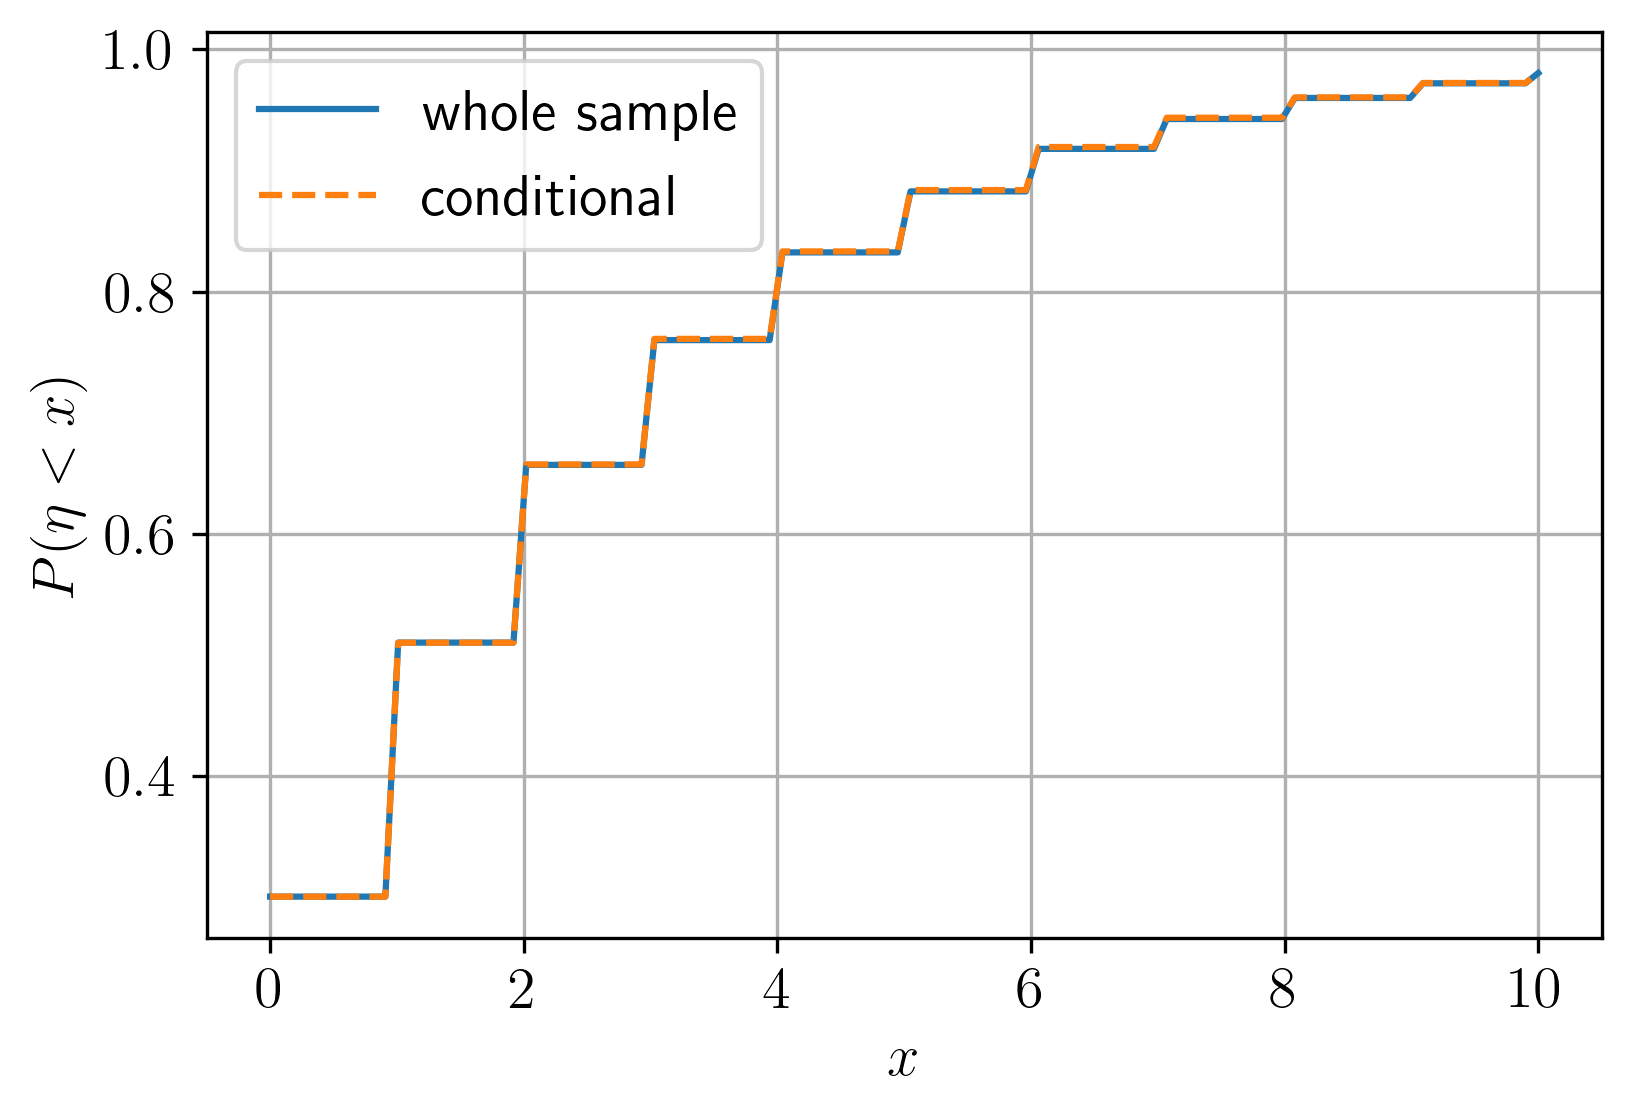
\includegraphics[width=0.5\textwidth]{figures/01_mem.png}
    \caption{Свойство отсутствия памяти для геометрического распределения.}
    \label{fig:01_mem}
\end{figure}
На графике отчетливо видно наложение двух эмпирических функций распределения.

Для 3 части задания одна из траекторий для игры в орлянку:

\begin{figure}[H]
    \centering
    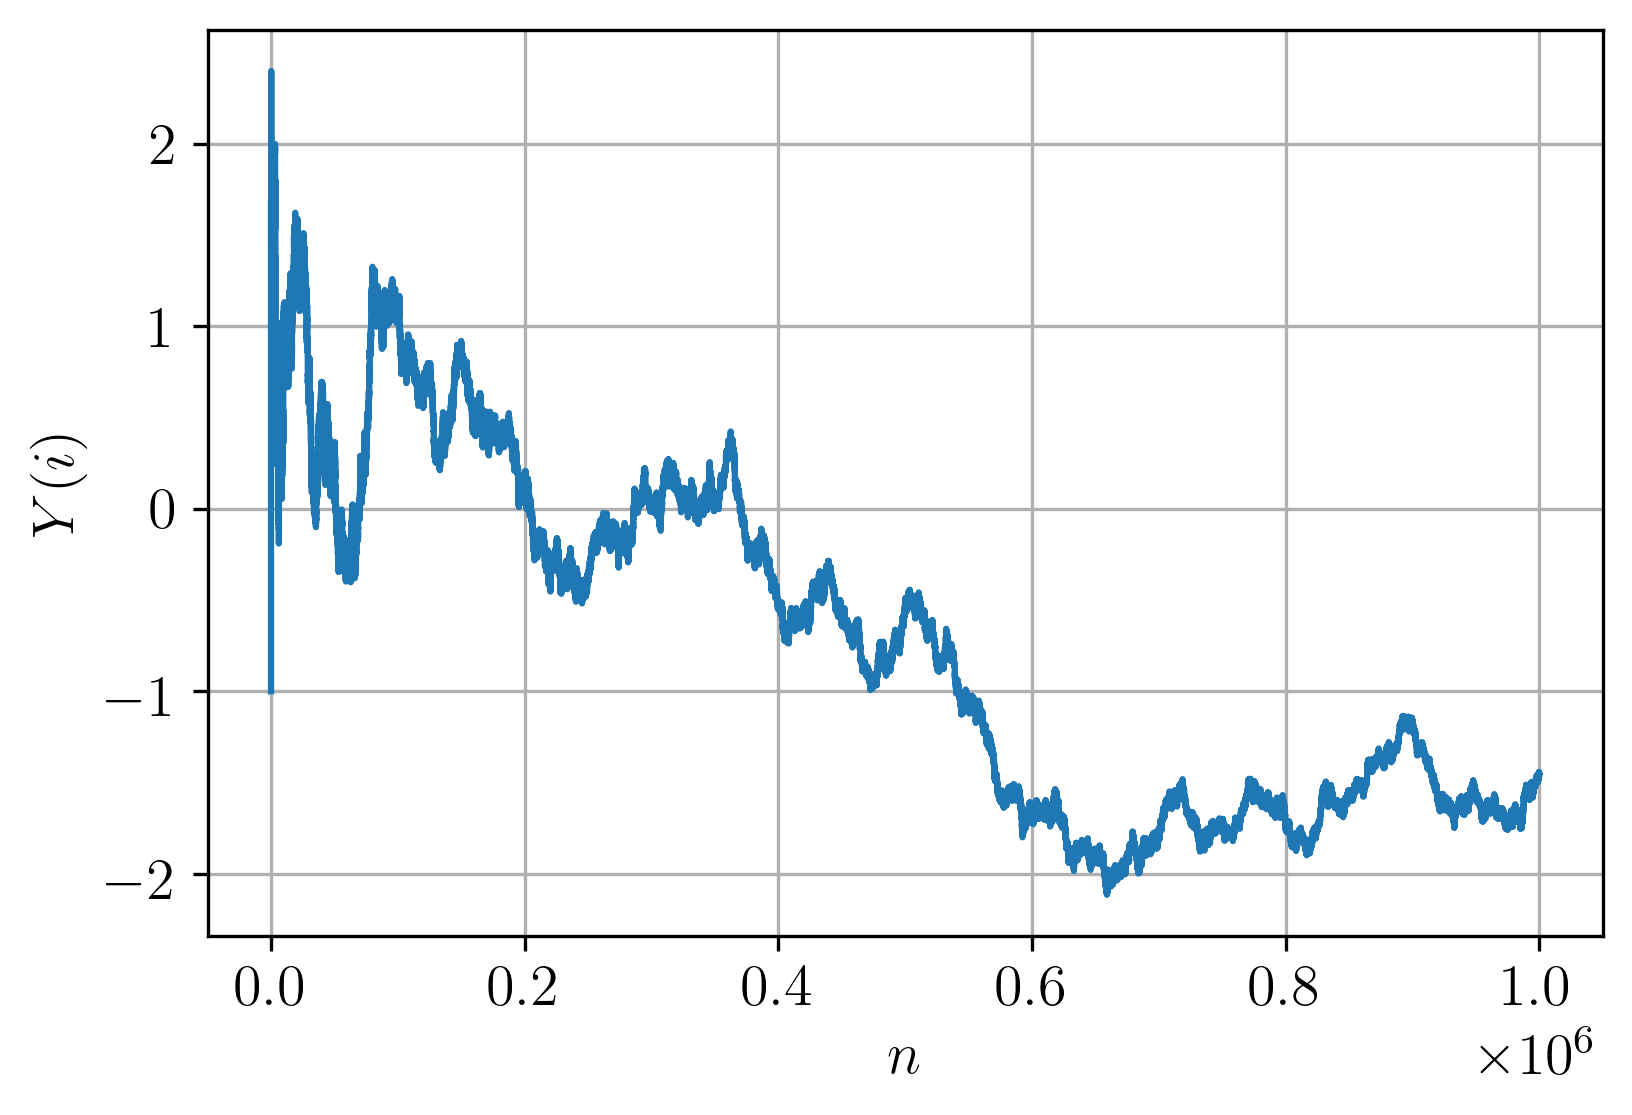
\includegraphics[width=0.5\textwidth]{figures/01_coin.png}
    \caption{Одна из возможных траекторий $Y(i)$ при игре в орлянку.}
    \label{fig:01_coin}
\end{figure}


\section{Задание 2}

\subsection{Постановка задачи}

\begin{enumerate}
\item Построить датчик сингулярного распределения, имеющий в качестве функции распределения канторову лестницу. С помощью критерия Колмогорова убедиться в корректности работы датчика.
\item Для канторовых случайных величин проверить свойство симметричности относительно 0.5 и самоподобия относительно деления деления на 3 с помощью критерия Смирнова.
\item Вычислить значение матожидания и дисперсии для данного распределения. Сравнить теоретические и эмпирические значения, проиллюстрировать сходимость.
\end{enumerate} 

\subsection{Теоретическая часть}

\begin{Def}
    Канторовой лестницей нахывается функция $f$, которая строится следующим образом:
    \begin{enumerate}
        \item $f(0) = 0$,  $f(1) = 1$.
        \item Отрезок  $[0, 1]$ разбивается на 3 равных части, затем на 
            средней части функция  $f$ полагается равной полусумме значений на концах.
        \item для первого и третьего отрезка процедура повторяется рекурсивно.
    \end{enumerate} 
\end{Def} 

По определению канторова лестница обладает свойством фрактальности или самоподобия:
$f(x) = 2f(x / 3)$.
Так как  $f$ монотонна и лежит в отрезке  $[0, 1]$, то существует 
случайная величина $X$ (сингулярная), функция распределения которой является канторовой лестницей.

Используя свойство фрактальности данной случайной величины, найдем ее математическое ожидание и дисперсию:
\[
    X \Eqtext{d} 1 - X \implies \Expec X = 0.
\] 
\begin{equation*}
    \Expec X^2 = \int\limits_{0}^{1} x^2 dF(x) = 
    \int\limits_{0}^{\frac{1}{3}} x^2 dF(x) +
    \int\limits_{\frac{2}{3}}^{1}  x^2 dF(x).    
\end{equation*}
Отсюда используя замену $y = 3x$ и свойство $F(x / 3) = F(x) / 2$ получаем 
 \[
     \var\left[ X \right] = \Expec X^2 = \frac{3}{8}.
\] 

Для проверки свойств распределения будем использовать критерии Колмогорова и Смирнова.
В тесте Колмогорова проверяется гипотеза $H_0\colon F = F_0$ соответствия распределения некоторому наперед заданному распределению  $F_0$.
Для проверки гипотезы строится следующая статистика:
 \[
     D_n = \sup\limits_x \bigl\lvert F_n(x) - F_0(x) \bigr\rvert, 
\]
где $F_n(x)$~---~эмпирическая функция распределения, потстроенная по выборке  $X_1, \ldots, X_n$.
Теорема Колмогорова утверждает, что $\sqrt{n}D_n \xrightarrow[n \rightarrow \infty]{d} K$, 
где  $K$~---~распределение Колмогорова.
Зафиксируем некоторый уровень доверия  $\alpha$ и будем отклонять гипотезу, когда
\[
    \sqrt{n} D_n > K^{-1}(1 - \alpha).
\] 

Для проверки гипотезы о принадлежности двух выборок размеров $m$ и  $n$ к одному распределению используется следующая статистика:
 \[
     D_{mn} = \sup\limits_x \bigl\lvert F_n(x) - G_m(x) \bigr\rvert,
\] 
где $F_n$ и  $G_m$~---~эмпирические функции распределения.
По теореме Смирнова 
 \[
     \sqrt{\frac{mn}{m+n}}D_{mn} \xrightarrow[n\rightarrow \infty]{d} K,
\] 
поэтому при больших размерах выборки ($m, n > 20$) отклоняем гипотезу, если 
\[
    \sqrt{\frac{mn}{m+n}}D_{mn} > K^{-1}(1 - \alpha).
\] 

\subsection{Результаты работы программы}

\begin{figure}[H]
    \centering
    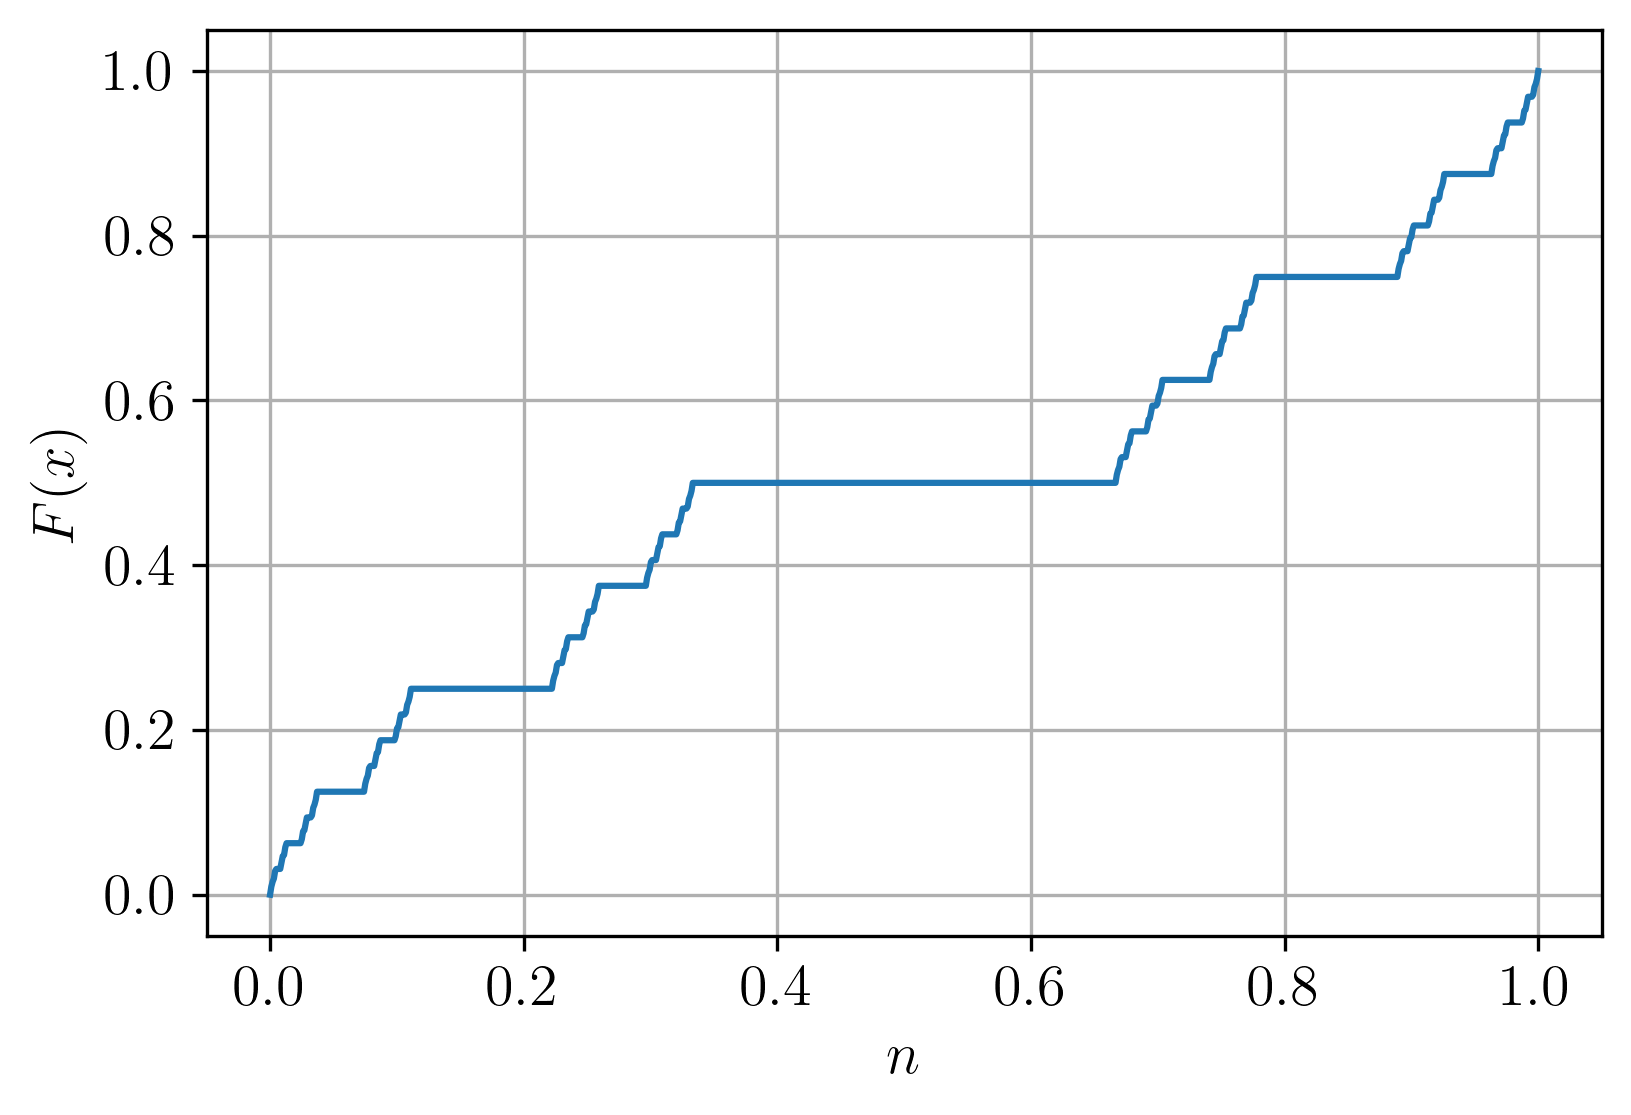
\includegraphics[width=0.5\textwidth]{figures/02_cdf.png}
    \caption{Функция распределения канторовой лестницы.}
    \label{fig:02_cdf}
\end{figure}

\begin{figure}[H]
    \centering
    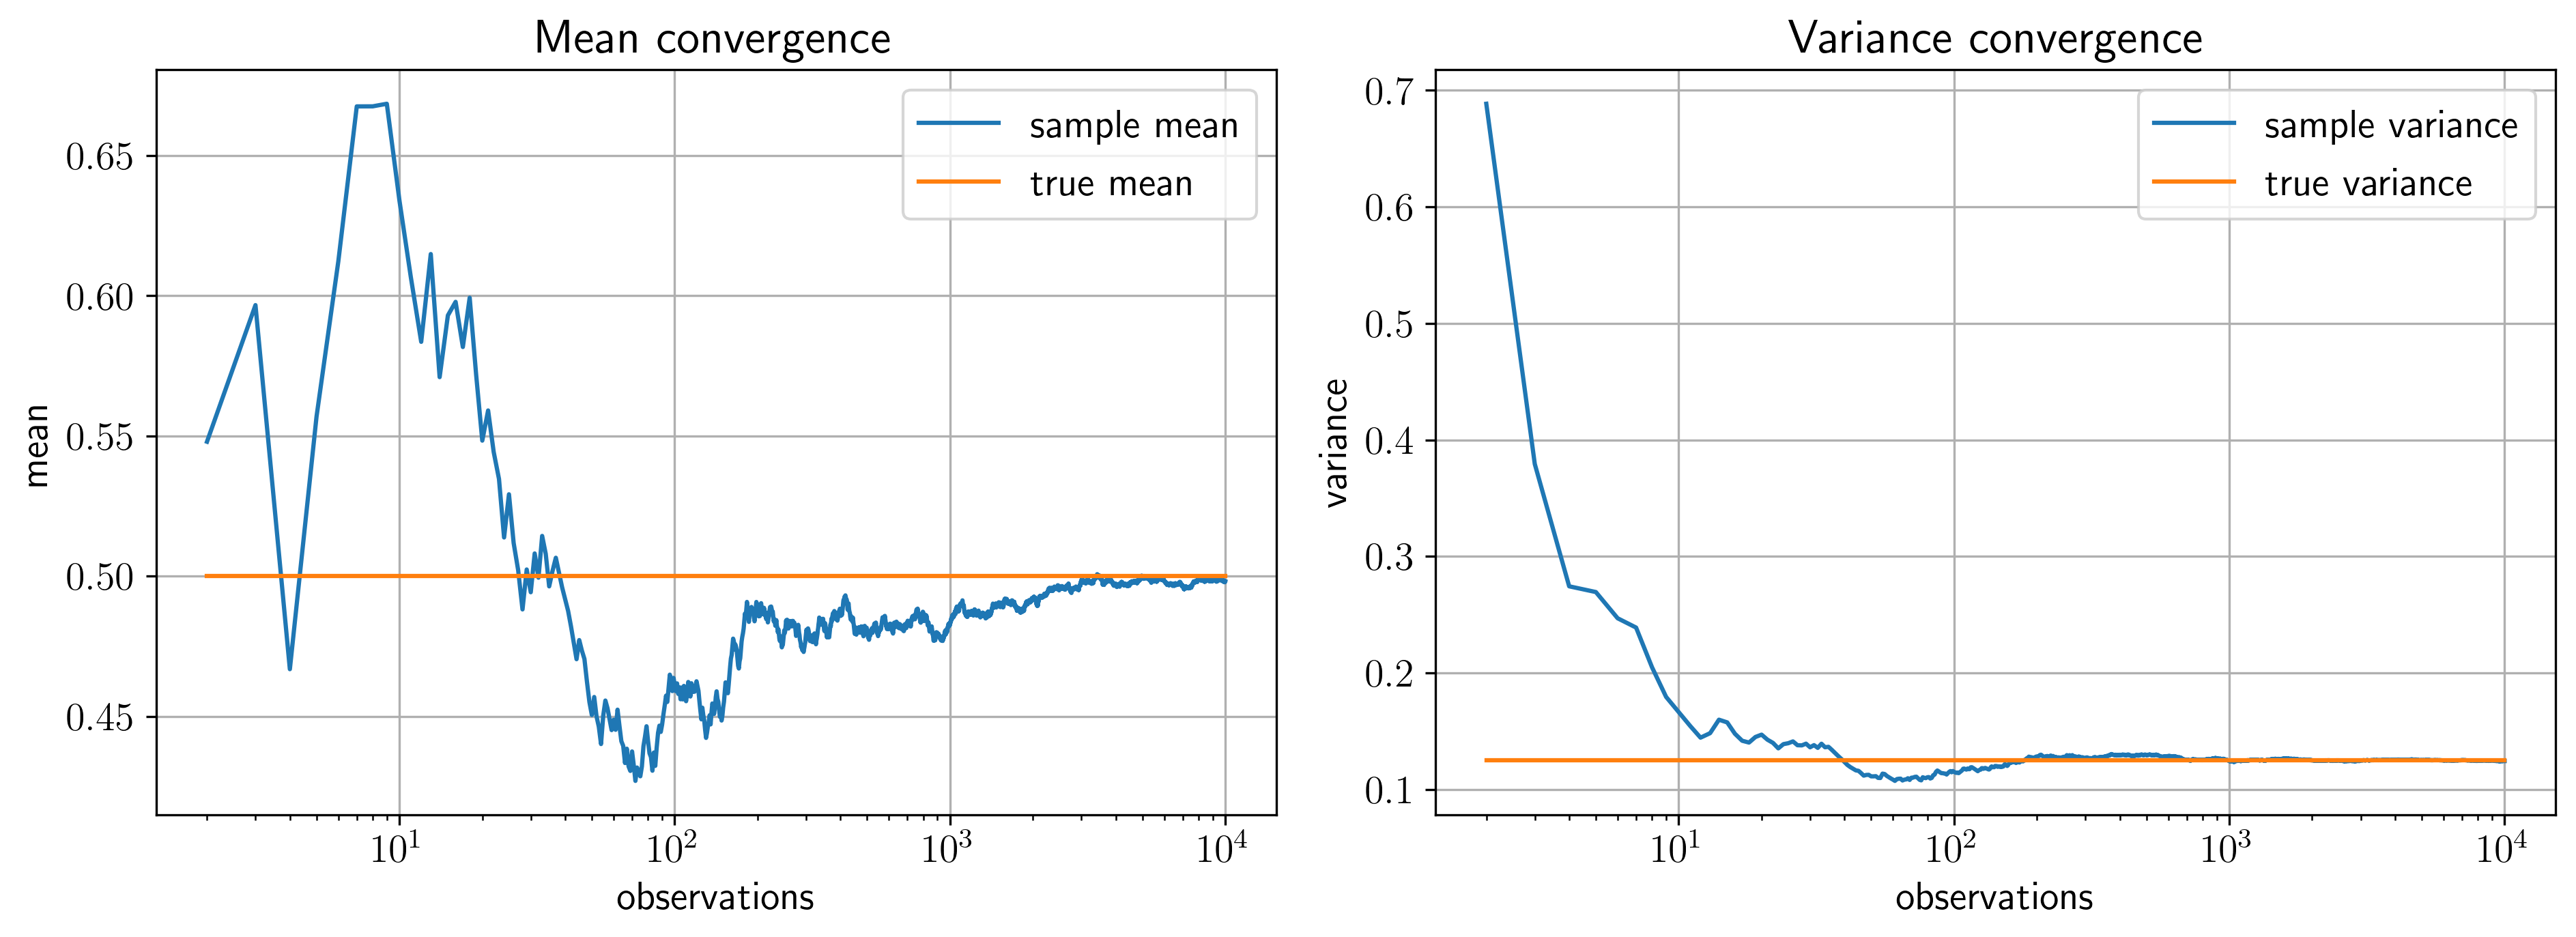
\includegraphics[width=\textwidth]{figures/02_conv.png}
    \caption{Иллюстрация сходимости статистик сингулярного распределения.}
    \label{fig:02_conv}
\end{figure}


\section{Задание 3}


\subsection{Постановка задачи}
\begin{enumerate}
\item Построить датчик экспоненциального распределения. Проверить для данного распределения свойство отсутствия памяти. 
    Пусть\par $X_1, \ldots, X_n$ независимы и имеют экспоненциальное распределение с параметрами $\lambda_1, \ldots, \lambda_n$. Найти распределение случайной величины $Y = \min(X_1, \ldots, X_n)$.
\item На основе датчика экспоненциального распределения построить датчик пуассоновского распределения.
\item Построить датчик пуассоновского распределения как предел биномиального. С помощью критерия хи-квадрат убедиться, что получен датчик распределения Пуассона.
\item Построить датчик стандартного нормального распределения методом моделирования случайных величин с переходом в полярные координаты. Проверить при помощи t-критерия Стьюдента равенство матожиданий, а при помощи критерия Фишера равенство дисперсий.
\end{enumerate}

\subsection{Теоретическая часть}

\begin{Def}
    Экспоненциальным распределением с параметром $\lambda$ будем называть 
    распределение с плотностью $p(x) = \lambda e^{-\lambda x}$.
\end{Def} 
\begin{St}
    Экспоненциальное распределение обладает свойством отсутствия памяти:
    $$
    \Pro (X \ge x + y \mid X \ge y) \hm= \Pro(X \ge x).
    $$
\end{St} 
\begin{Proof}
    \begin{equation*}
        \Pro (X \ge x + y \mid X \ge y) = 
        \frac{e^{-\lambda (x + y)}}{e^{-\lambda y}} = e^{-\lambda x} = 
        \Pro(X \ge x).
    \end{equation*}
\end{Proof} 

Рассмотрим еще одно свойство экспоненциального распределения.
Пусть $X_1, \ldots , X_n$ нещависимы и распределены экспоненциально с
показателями $\lambda_1,\ldots \lambda_n$ соответственно.
Пусть также $Y = \min \left\{ X_1,\ldots , X_n \right\}$.
Тогда 
\[
    F_Y(x) =\Pro(Y < x) = 
    1 - \Pro\left( X_1 \ge x,\ldots , X_n \ge x \right) =
    1 - \prod\limits_{i=1}^{n} e^{-\lambda_i x} =
    1 - e^{-x\sum\limits_{i=1}^{n} \lambda_i}.
\] 
Таким образом, $Y$ распределена экспоненциально с показателем  $\sum\limits_{i=1}^{n} \lambda_i$.

Рассмотрим два способа моделирования распределения Пуассона.
Первый заключается в том, что промежутки между скачками пуассоновского 
процесса с параметром $\lambda$ распределены экспоненциально, 
а случайная величина  $X(1)$ имеет распределение Пуассона с параметром  $\lambda$.

Второй способ дает 
\begin{Th}[Пуассона]
    Пусть в схеме серий испытаний Бернулли с вероятностями $p_n$ выполнено:
     \[
        p_n \xrightarrow[n \rightarrow\infty]{} 0,\qquad 
        np_n \xrightarrow[n \rightarrow \infty]{} \lambda > 0.
    \]
    Тогда число успехов сходится к распределению Пуассона с параметром $\lambda$.
    При этом верна оценка:
     \[
         \left\lvert \Pro(S_n \in A) - \sum\limits_{k \in A} e^{-\lambda} \frac{\lambda^{k}}{k!}  \right\rvert \le \lambda p.
    \] 
\end{Th}
Чтобы получить вероятность, отличающуюся от распределения Пуассона не больше чем на $\epsilon$,
положим  $p = \frac{\epsilon}{\lambda}$ и $n = \frac{\lambda^2}{\epsilon}$. 
Тогда биномиальное распределение с такими параметрами будет хорошо приближать распределение Пуассона.

Для моделирования стандартного нормального распределения рассмотрим пару случайных величин $(X_1, X_2)$,
которую будем рассматривать, как двумерный вектор.
Пусть  $(r, \phi)$~---~запись вектора в полярных координатах.
Из симметрии $\phi \sim U[0, 2\pi]$.
Из свойств нормального распределения  $r^2 \sim exp(\frac{1}{2})$.
Тогда моделируя угол равномерным распределением и квадрат радиуса экспоненциальным, 
будем получать 2 стандартных нормальных случайных величины после перехода в декартовы координаты.

Критерий $\chi^2$ Пирсона используется для проверки гипотезы равенства распределения заданному $H_0\colon F = F_0$. 
Разобьем прямую на непересекающиеся части $\Delta_1,\ldots \Delta_m$ и
положим $p_i = \Pro(X \in \Delta_i \mid H_0)$.
Обозначим за $N_i$ число элементов выборки, попавших в $\Delta_i$.
Тогда статистика 
 \[
     Q = \sum\limits_{i=1}^{m} \frac{(N_i - np_i)^2}{np_i}
     \sim \chi^2_{m-1}.
\] 
Тогда отклоняем гипотезу, если $\chi^2_{m-1}(Q) < \alpha$.

Пусть дана выборка $X_1,\ldots X_n$ из нормального распределения с неизвестными параметрами.
Для проверки гипотезы $H_0\colon \Expec X = \mu$ используется критерий Стьюдента. 
Положим 
\[
    \hat{\sigma} = \sqrt{\frac{1}{n - 1} \sum\limits_{i=1}^{n} \left( X_i - \overline{X} \right)^2}.
\] 
Тогда статистика 
\[
    U = \sqrt{n} \frac{\overline{X} - \mu}{\hat{\sigma}}
    \sim St_{n-1}.
\] 
Будем отклонять гипотезу, если $St_{n-1}(U) < \frac{\alpha}{2}$.

Для сравнения дисперсий двух нормально распределенных выборок используется критерий Фишера.
Пусть даны две выборки $X_1,\ldots ,X_n$ и  $Y_1,\ldots Y_m$. 
Тогда 
\[
    V = \frac{(m-1)\sum\limits_{i=1}^{n} (X_i - \overline{X})^2}{(n-1)\sum\limits_{i=1}^{m} (Y_i - \overline{Y})^2}
    \sim F_{m-1, n-1}.
\] 
Гипотеза отвергается, если $F_{m-1,n-1}(V) < \frac{\alpha}{2}$.

\subsection{Результаты работы программы}

Иллюстрацию свойства отсутствия памяти проведем аналогично с 1-м заданеим:
\begin{figure}[H]
    \centering
    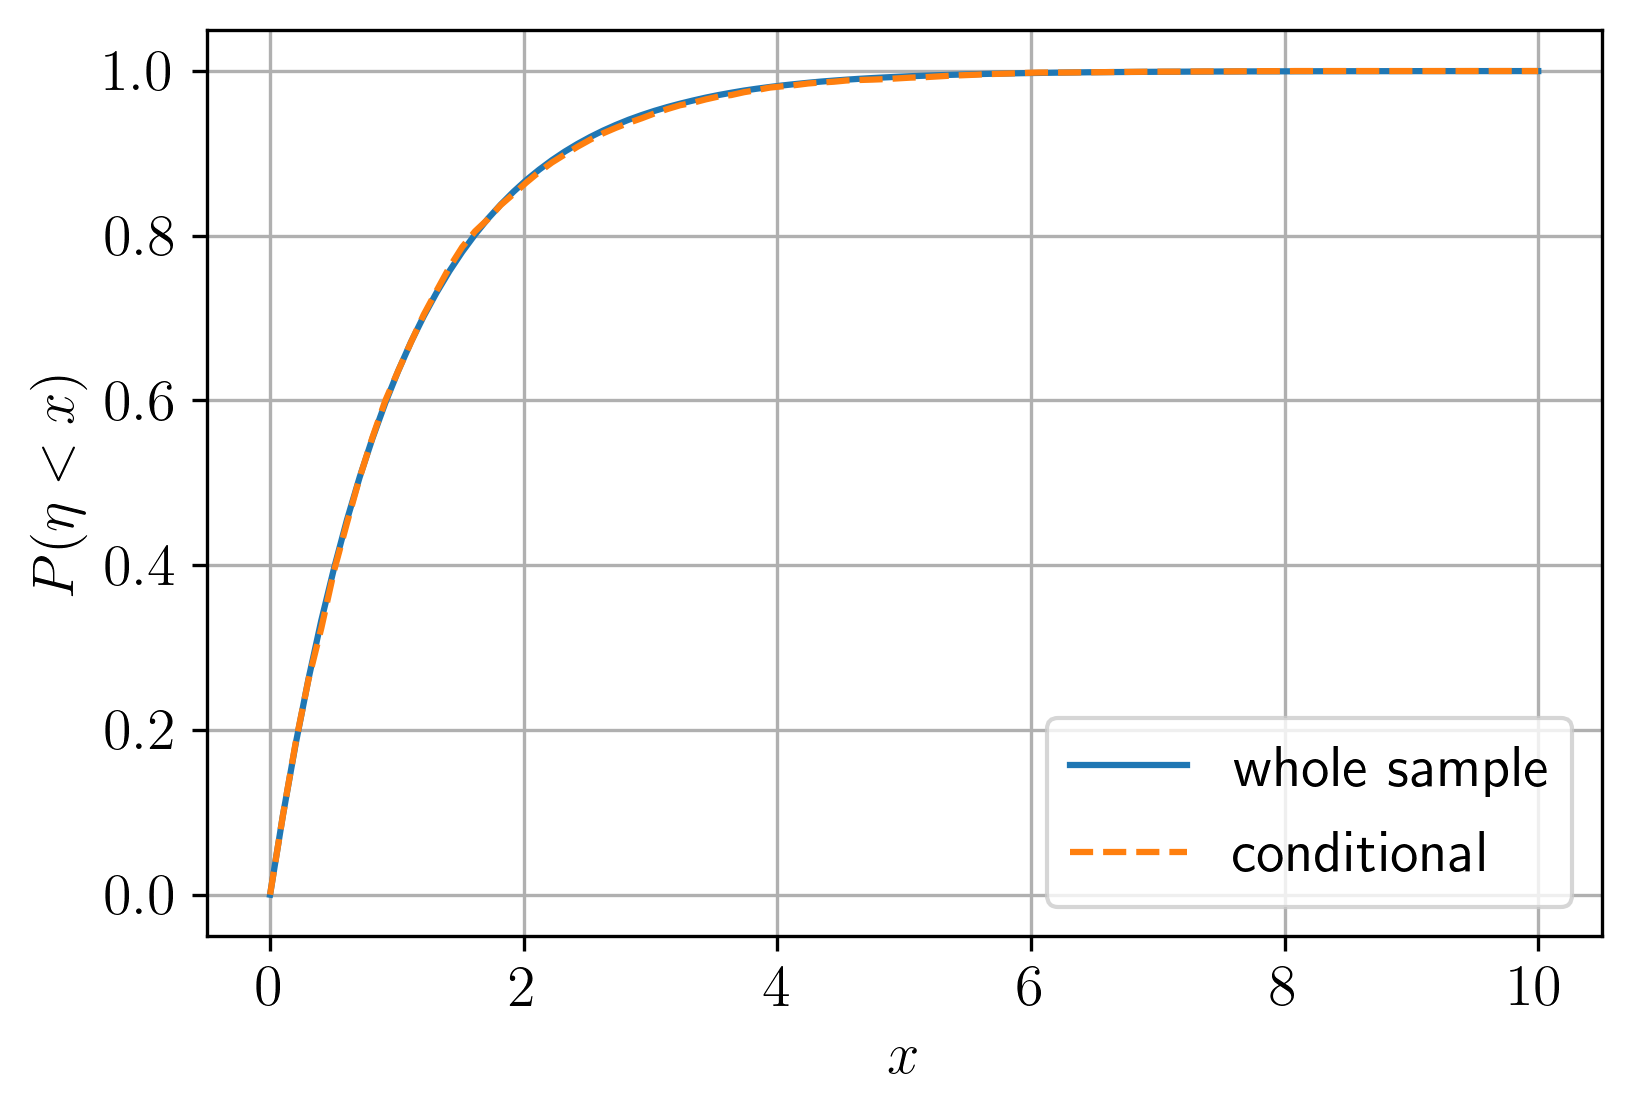
\includegraphics[width=0.5\textwidth]{figures/03_mem.png}
    \caption{Свойство отсутствия памяти для экспоненциального распределения.}
    \label{fig:03_mem}
\end{figure}

Распределения минимума случайных величин проиллюстрируем, 
наложив на один график эмпирическую и теоретическую функции распределения (размер выборки $1000$ для каждой из  $100$ случайных величин):
\begin{figure}[H]
    \centering
    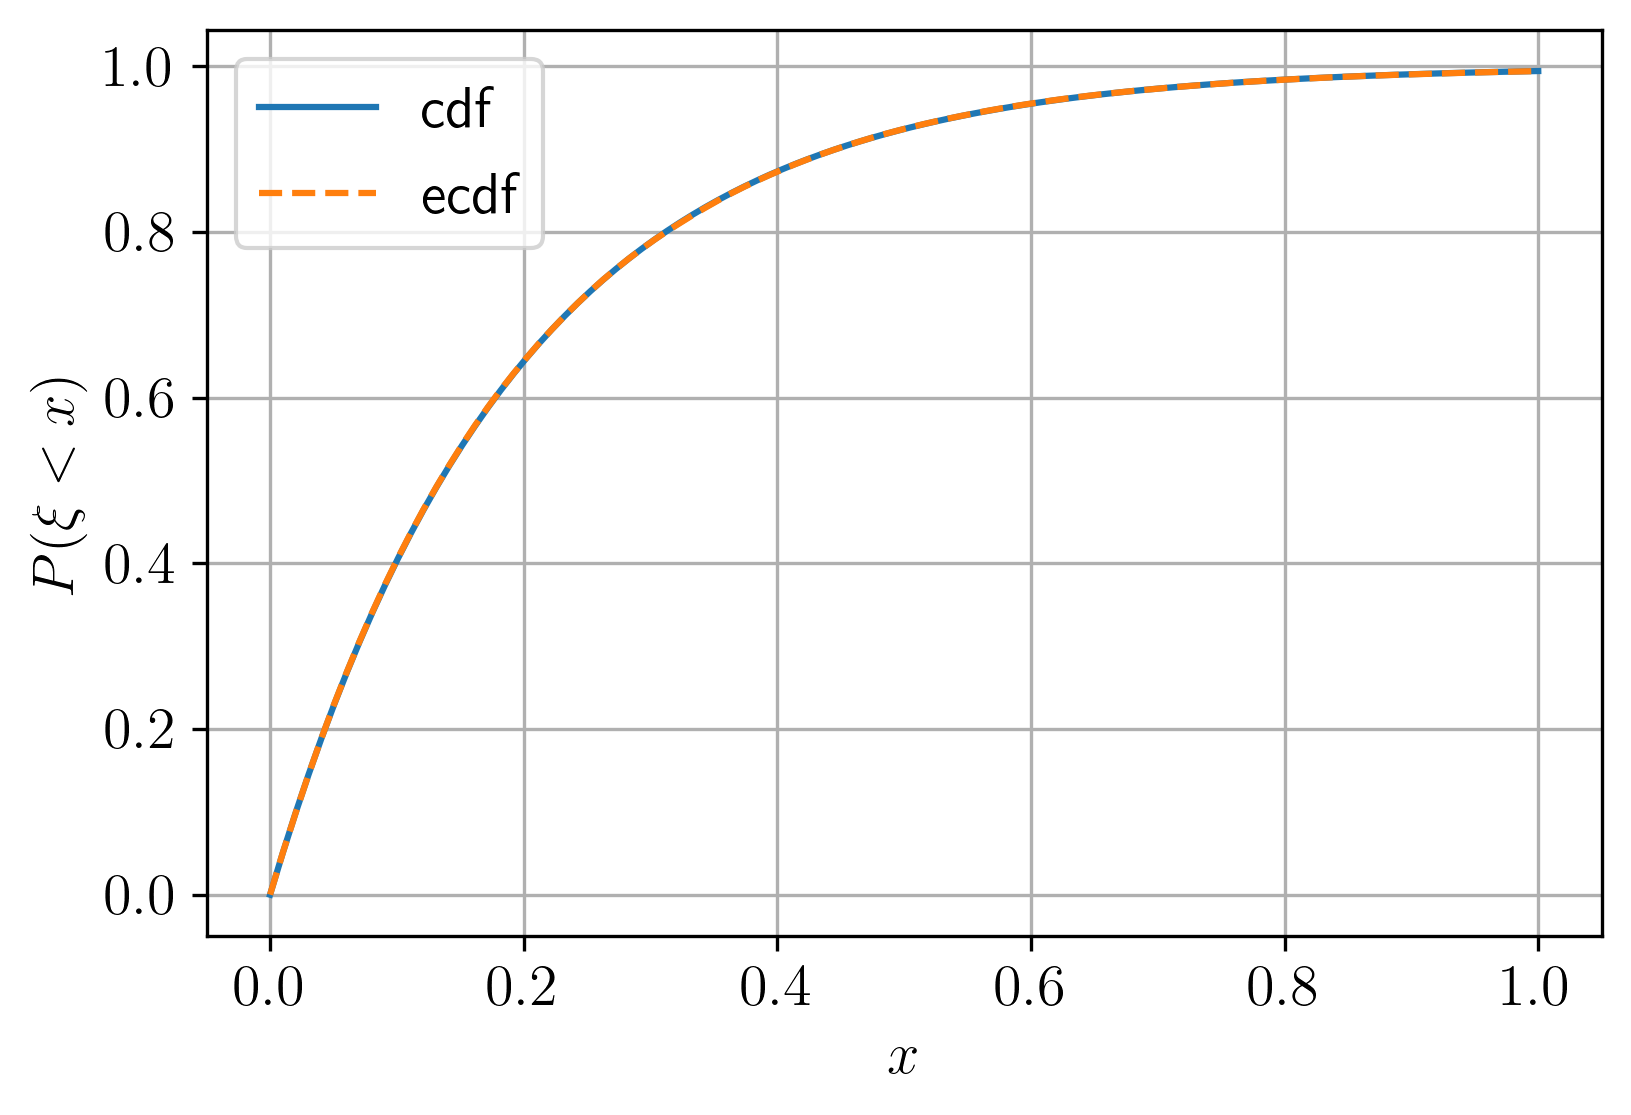
\includegraphics[width=0.5\textwidth]{figures/03_cdfmin.png}
    \caption{Распределение минимума.}
    \label{fig:03_cdfmin}
\end{figure}

При проверке гипотез были получены следующие результаты (выборка генерировалась $1000$ раз):

\begin{tabular}[H]{ccc}
    Критерий & Частота отклонения & Уровень значимости \\
    Хи-квадрат & $3{,}0\%$ &  $0{,}95$ \\
    Стьюдента &  $3{,}0\%$ &  $0{,}95$ \\
    Фишера & $6{,}0\%$ & $0{,}95$
\end{tabular} 

\section{Задание 4}
\subsection{Постановка задачи}
\begin{enumerate}
\item Построить датчик распределения Коши.
\item На основе датчика распределения Коши с помощью метода фон Неймана построить датчик стандартного нормального распределения. При помощи norm probability plot убедиться в корректности построенного датчика и обосновать наблюдаемую линейную зависимость.
\item Сравнить скорость моделирования стандартного нормального распределения в заданиях 3 и 4.
\end{enumerate}  

\subsection{Теоретическая часть}

\begin{Def}
    Случайная величина $\xi$ имеет распределение Коши с параметрами  $a, b$
    ($\xi \sim \mathcal{C}(a, b)$), 
    если ее функция распределения имеет вид:
    \[
        F_\xi(x) = \frac{1}{2} + \frac{1}{\pi} \arctg\left( \frac{x - a}{b} \right).
    \] 
\end{Def} 
    Для моделирования распределения Коши, воспользуемся методом обращения 
    функции распределения:
    \[
        F^{-1}(y) = a + b \tg\left( \pi \left( y - \frac{1}{2} \right) \right).
    \] 

Метод элиминации фон Неймана подробно описан в~\cite{Bishop}.
В нашем случае:
\[
    p(x) = e^{-\frac{x^2}{2}},\quad 
    q(x) = \frac{b}{\pi \left[ (x - a)^2 + b^2 \right]}.
\]
Наилучшие результаты в смысле частоты отклонения дают параметры $a=0,\ b=1$.
Тогда:
 \[
     k = \sup_x \frac{p(x)}{q(x)} = \frac{2}{\sqrt e}.
\] 
Затем будем генерировать случайные величины $\xi_n \sim Q$.
Каждое значение в полученной выборке будем отбирать в конечную выборку с вероятностью  $p(\xi_k) \big/ kq(\xi_k)$.

Для тестирования полученного датчика воспользуемся norm probability plot.
По определению для norm probability plot ось ординат деформируется таким образом,
чтобы функция распределения для стандартной гауссовской случайной величины была линейна.
Тогда если дана выборка из распределения с параметрами $\mu, \sigma$,
то это эквивалентно сдвигу графика стандартного распределения на $\mu$ вправо вдоль оси абсцисс и уменьшению углового коэффициента в $\sigma$ раз.
\subsection{Результаты работы программы}

Результат работы алгоритма фон Неймана: 
\begin{figure}[H]
    \centering
    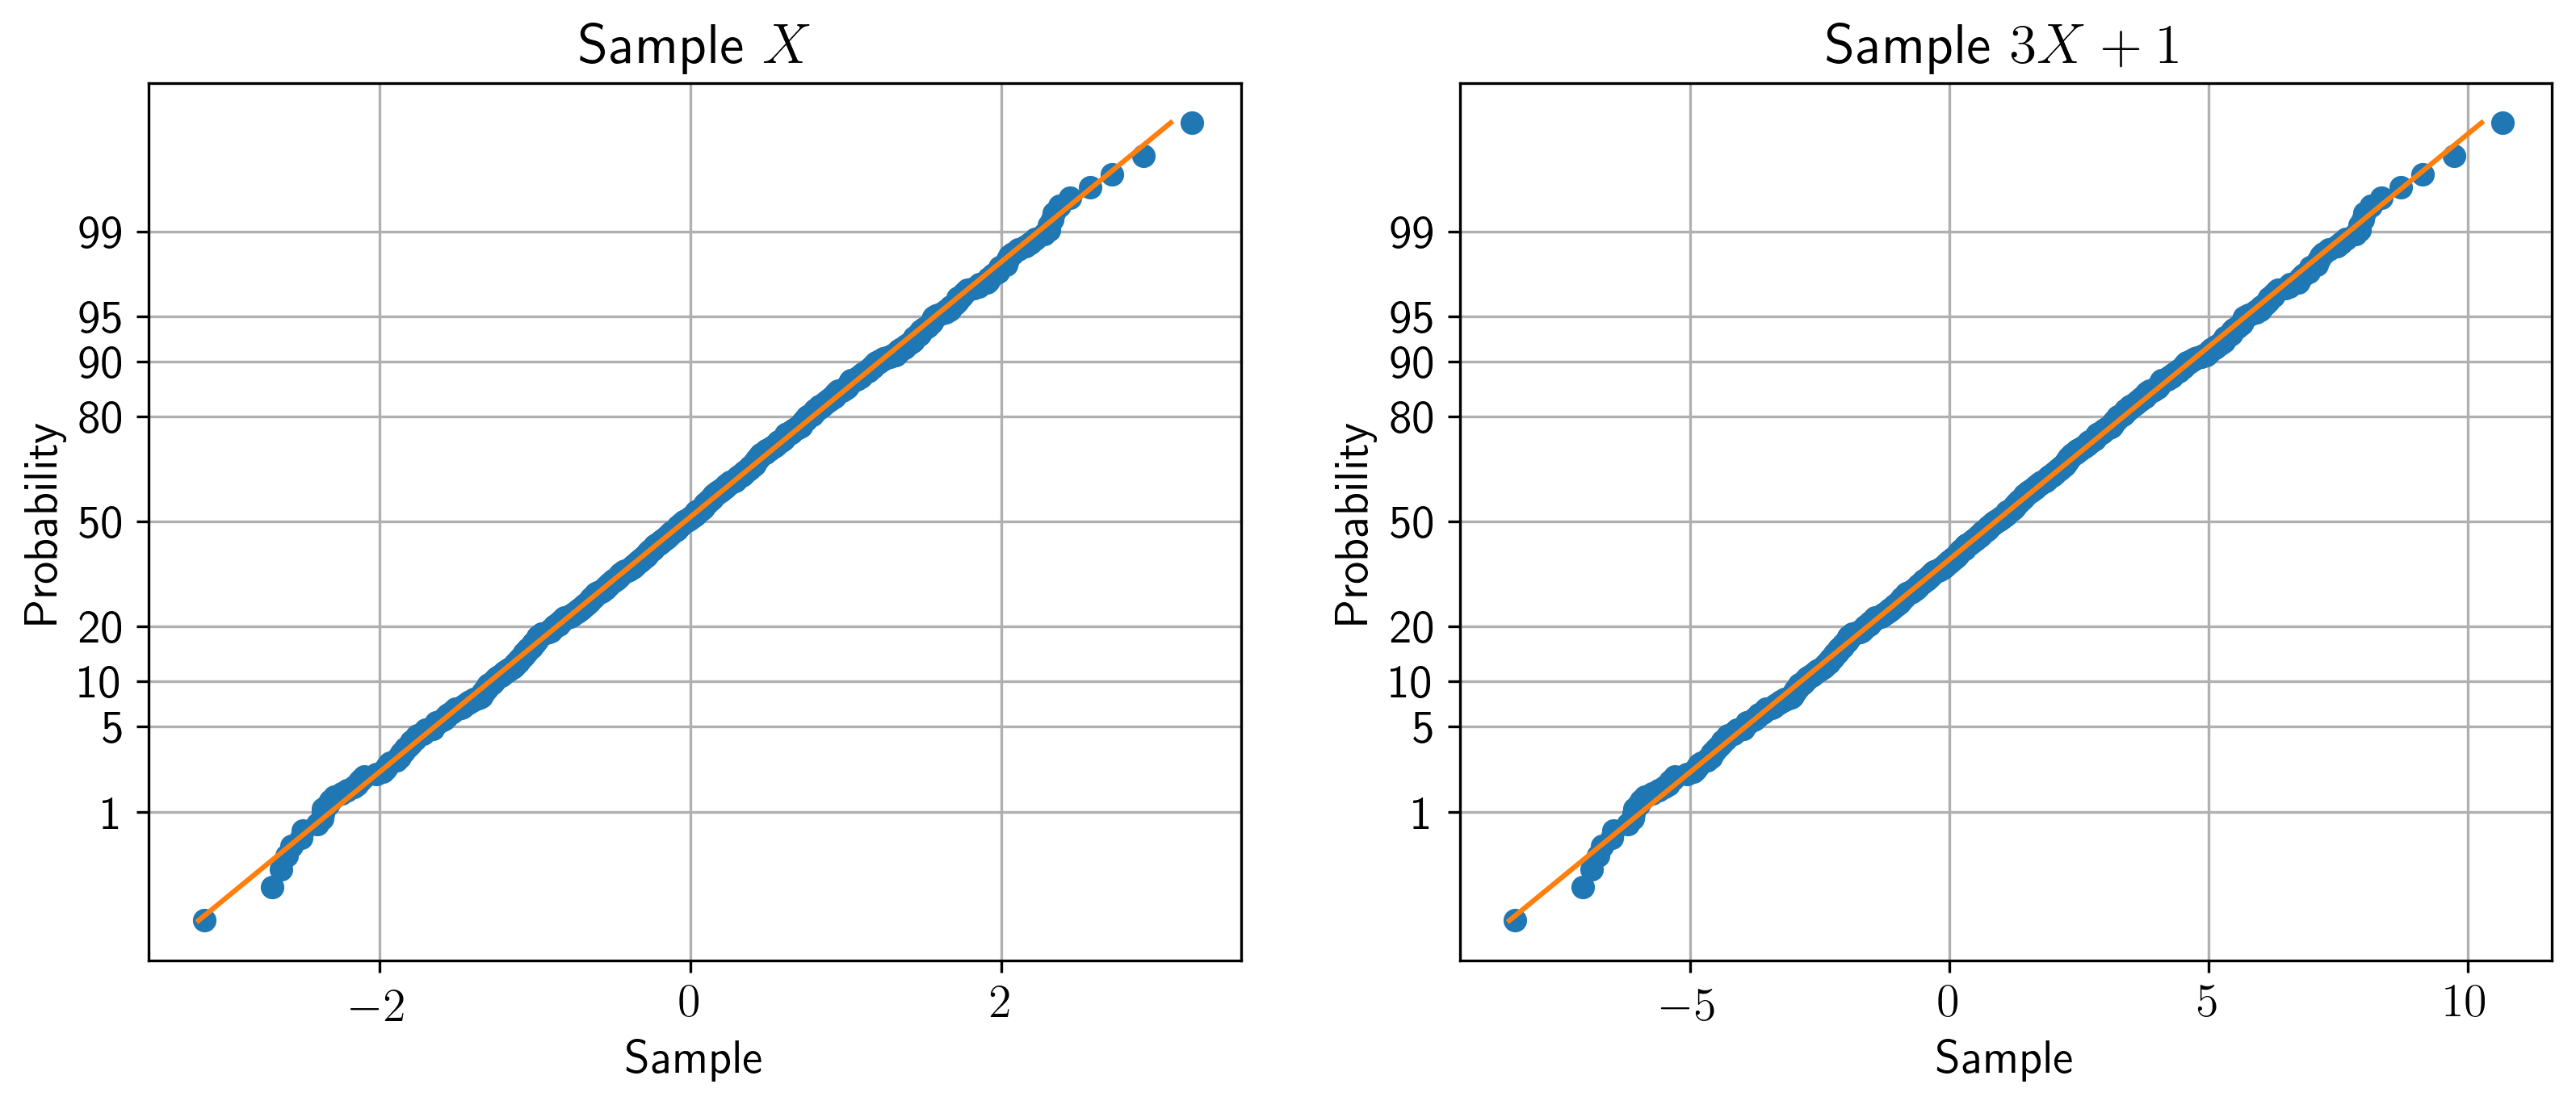
\includegraphics[width=\textwidth]{figures/04_normplot.png}
    \caption{Normal probability plot.}
    \label{fig:04_normplot}
\end{figure}

Для сравнения скорости работы алгоритмов были сгенерированы выборки разного размера. 
Для каждого размера выборка генерировалась $10$ раз, 
и в качестве итогового времени бралась медиана.
 \begin{figure}[H]
    \centering
    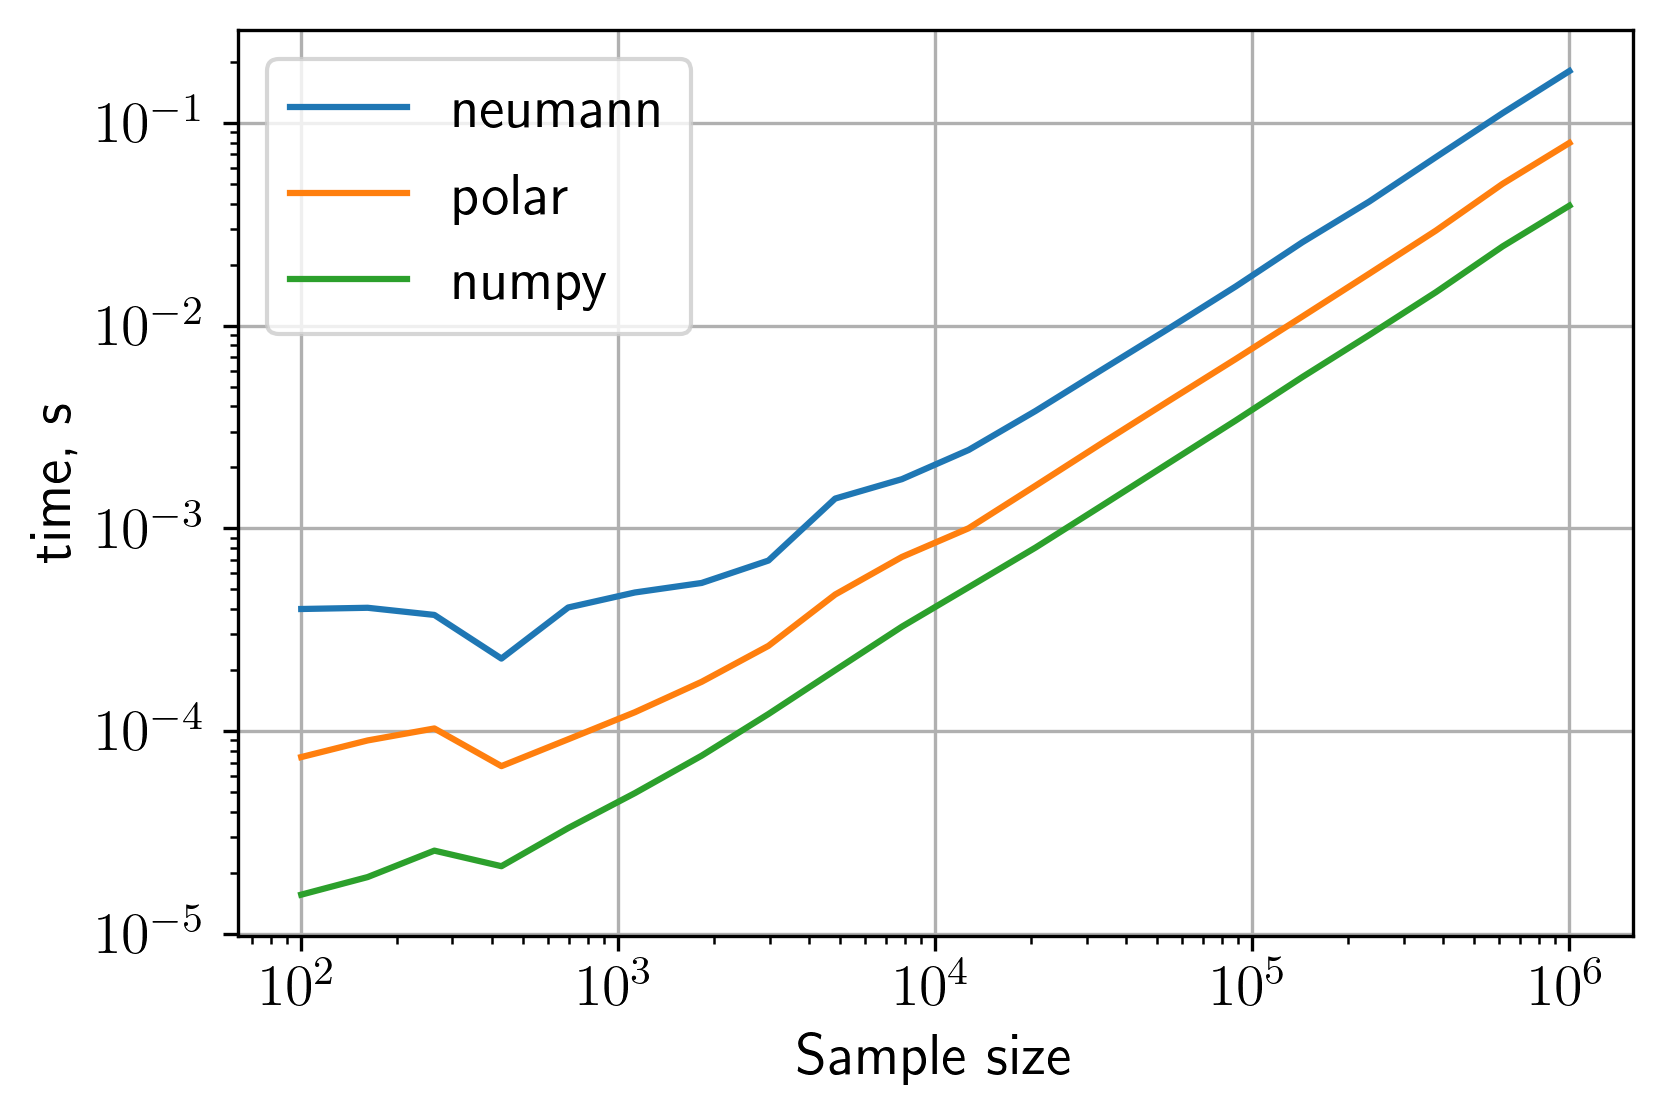
\includegraphics[width=0.5\textwidth]{figures/04_times.png}
    \caption{Сравнение скорости работы алгоритмов генерирования выборки из нормального распределения.}
    \label{fig:04_times}
\end{figure}


\section{Задание 5}
\subsection{Постановка задачи}

\begin{enumerate}
\item Пусть $X_i \sim \mathcal{N}(\mu, \sigma^2)$. Убедиться эмпирически в справедливости ЗБЧ и ЦПТ: исследовать поведение суммы $S_n$ и эмпирического распределения величины
$$\sqrt{n}\left(\frac{S_n}{n} - \mu\right).$$
\item Считая $\mu$ и $\sigma$ неизвестными, для пункта 1 построить доверительные интервалы для среднего и дисперсии.
\item Пусть $X_i \sim \mathcal{C}(a, b)$ имеет распределение Коши со сдвигом $a$ и масштабом $b$. Проверить эмпирически, как ведут себя суммы $\frac{S_n}{n}$. Результат объяснить, а также найти распределения данных сумм.
\end{enumerate}
\subsection{Теоретическая часть}

Сформулируем закон больших чисел и центральную предельную теорему.
\begin{Th}[УЗБЧ в форме Колмогорова]
Пусть $X_1, X_2, \ldots$ --- последовательность независимых одинаково распределенных случайных величин, имеющих конечные первые мометы. Тогда
\[
    \frac{1}{n} \sum\limits_{i=1}^{n} X_i \xrightarrow[n\rightarrow \infty]{\text{п.н.}} \Expec X_1.
\] 
\end{Th}

\begin{Th}[ЦПТ]
    Пусть $X_1, X_2,\ldots $~---~последовательность независимых одинаково распределенных случайных величин с конечным вторым моментом.
    Тогда 
    \[
        \sqrt n \left(\frac{S_n}{n}- \mu\right) \xrightarrow[n \rightarrow \infty]{d} \Norm(0, \sigma^2),
    \] 
    где 
    \[
        S_n = \sum\limits_{i=1}^{n} X_n, \quad 
        \mu = \Expec X_1, \quad \sigma^2 = \var X_1.
    \] 
\end{Th} 
Доказательства представлены в~\cite{Shir}.


Рассмотрим статистику $$U = \sqrt{n}\frac{\bar X - \mu}{\hat \sigma}, \quad \hat \sigma = \sqrt{\dfrac{\sum_{i=1}^n(X_i - \bar X)^2}{n-1}}$$
имеет \cite{DeGroot} распределение Стьюдента с $n - 1$ степенью свободы, можно построить доверительный интервал с уровнем доверия $\alpha$ следующим образом:
$$\mathbb{P}(\gamma_1 < U < \gamma_2) = \mathbb{P}\left(\bar X - \frac{\hat\sigma\gamma_2}{\sqrt{n}} < \mu < \bar X - \frac{\hat\sigma\gamma_1}{\sqrt{n}}\right) = \alpha.$$
Значения $\gamma_1$ и $\gamma_2$ выберем так, чтобы интервал был симметричным:
$$\gamma_1 = St^{-1}_{n-1}\left(\frac{1 - \alpha}{2}\right),\  \gamma_2 = St^{-1}_{n-1}\left(\frac{1 + \alpha}{2}\right).$$
Итак, доверительный интервал для параметра $\mu$ имеет вид
$$\left(\bar X - \frac{\hat\sigma\gamma_2}{\sqrt{n}}, \ \bar X - \frac{\hat\sigma\gamma_1}{\sqrt{n}}\right).$$

Для оценки дисперсии будем использовать статистику
$$V = \frac{\sum_i(X_i - \bar X)^2}{\sigma^2} \sim \chi^2(n - 1).$$
$$\mathbb{P}(\gamma_1 < V < \gamma_2) = \mathbb{P}\left(\frac{\sum_i(X_i - \bar X)^2}{\gamma_2} < \sigma^2 < \frac{\sum_i(X_i - \bar X)^2}{\gamma_1}\right) = \alpha.$$
Для построения симметричного интервала положим 
$$\gamma_1 = \left(\chi^2_{n-1}\right)^{-1}\left(\frac{1-\alpha}{2}\right), \ \gamma_2 = \left(\chi^2_{n-1}\right)^{-1}\left(\frac{1+\alpha}{2}\right).$$
Доверительный для $\sigma^2$ с уровнем доверия $\alpha$ имеет вид
$$\left(\frac{\sum_i(X_i - \bar X)^2}{\gamma_2}, \ \frac{\sum_i(X_i - \bar X)^2}{\gamma_1}\right).$$

Для оценки распределения суммы случайных величин, распределенных по Коши,
воспользуемся тем фактом, что распределение является устойчивым с показателем $1$.
Отсюда следует, что если $X_i \sim \mathcal{C}(a, b)$, то  
$\sum\limits_{i=1}^{n} X_i \sim \mathcal{C}(a, nb)$.

\subsection{Результаты работы программы}


\begin{figure}[H]
\begin{multicols}{2}
        \centering
        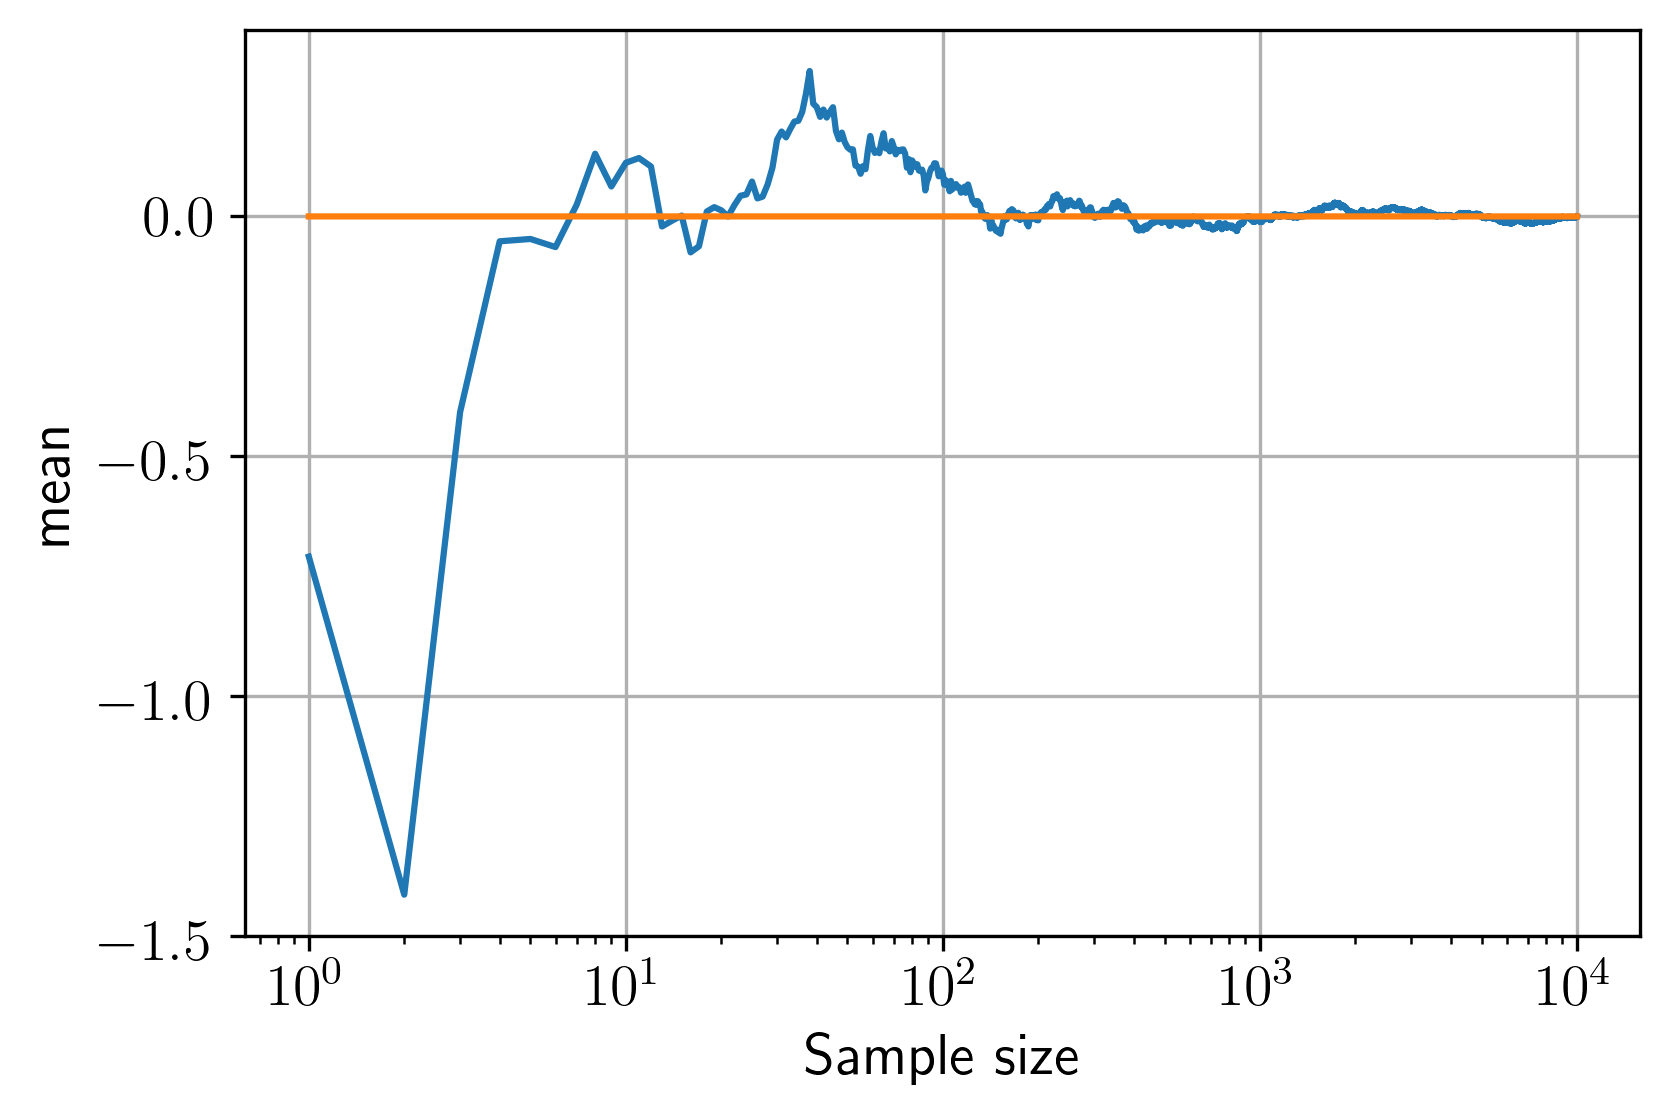
\includegraphics[width=0.5\textwidth]{figures/05_lln.png}
        \caption{Иллюстрация сходимости в ЗБЧ.}
        \label{fig:05_lln}
    \hfill
        \centering
        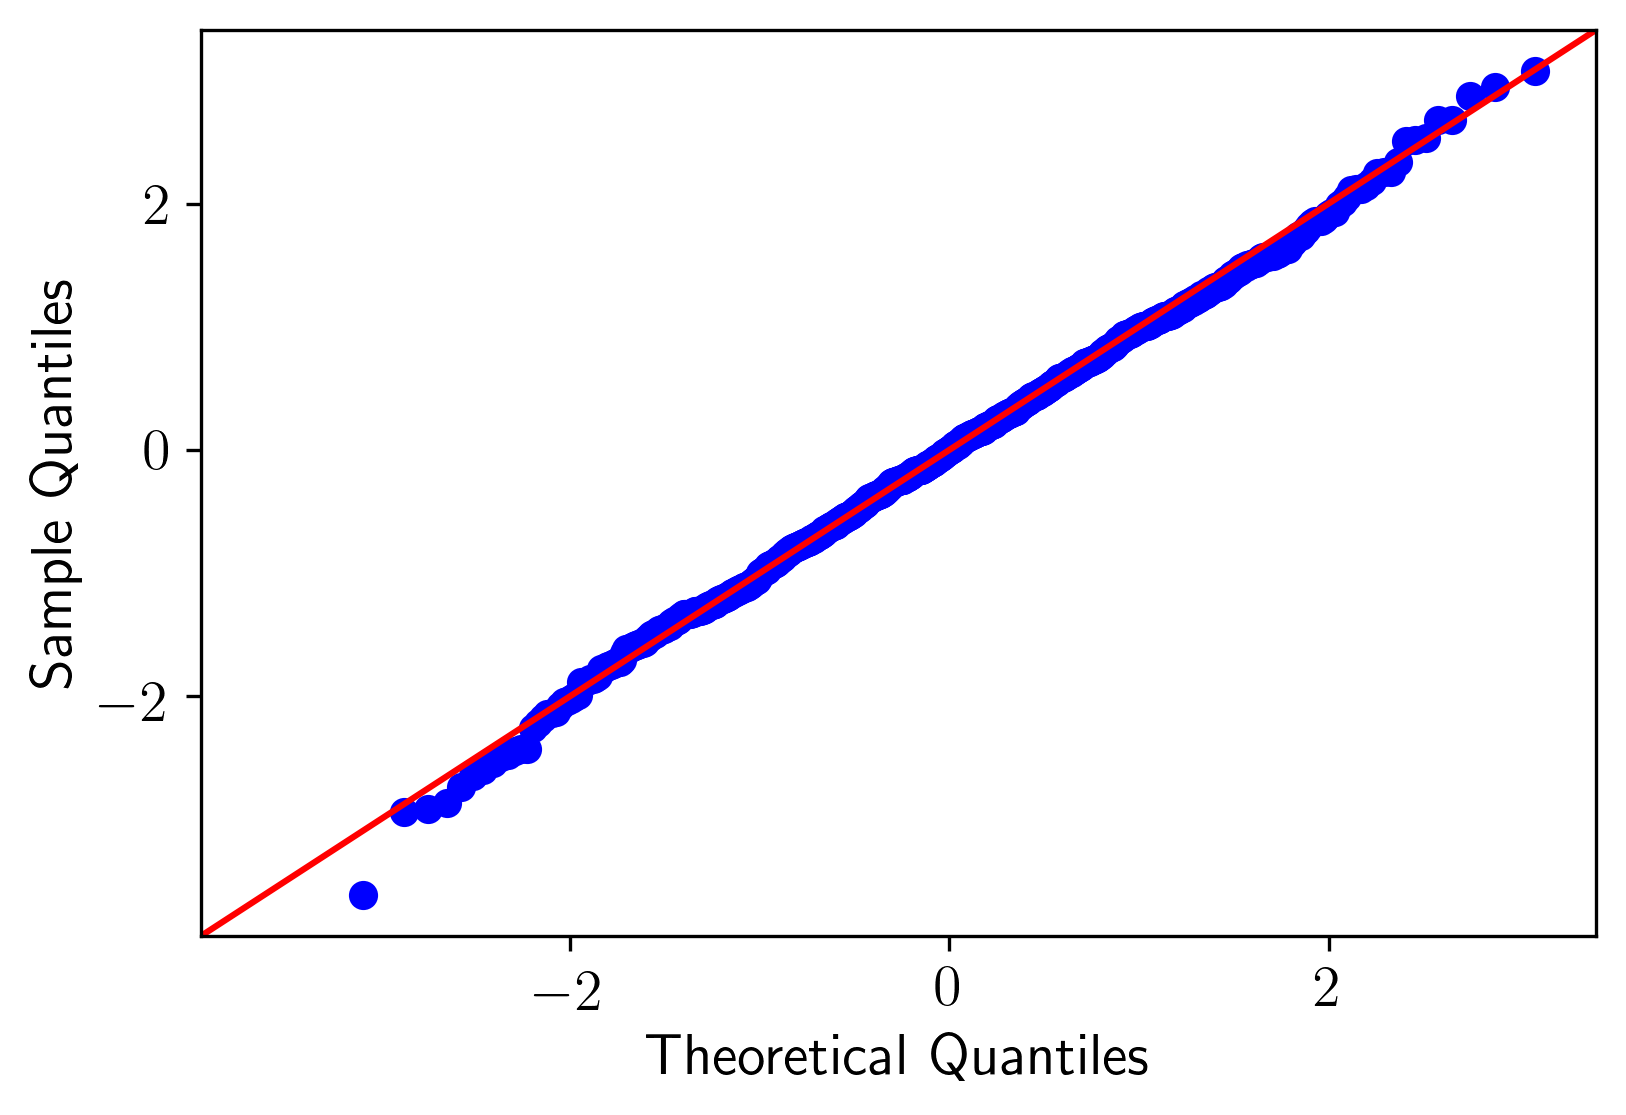
\includegraphics[width=0.5\textwidth]{figures/05_clt.png}
        \caption{Распределение нормированной суммы в ЦПТ при $n=1000$ (Q-Q plot).}
        \label{fig:05_clt}
\end{multicols} 
\end{figure}

На рис.~\ref{fig:05_lln} проиллюстрирована сходимость частичных сумм.
Предельное поведение частичных сумм видно из графика на рис.~\ref{fig:05_clt}.

На следующих двух рисунках построены графики с доверительными интервалами для математического ожидания и дисперсии выборки с уровнем значимости $\alpha = 0{,}95$.

\begin{figure}[H]
\begin{multicols}{2}
        \centering
        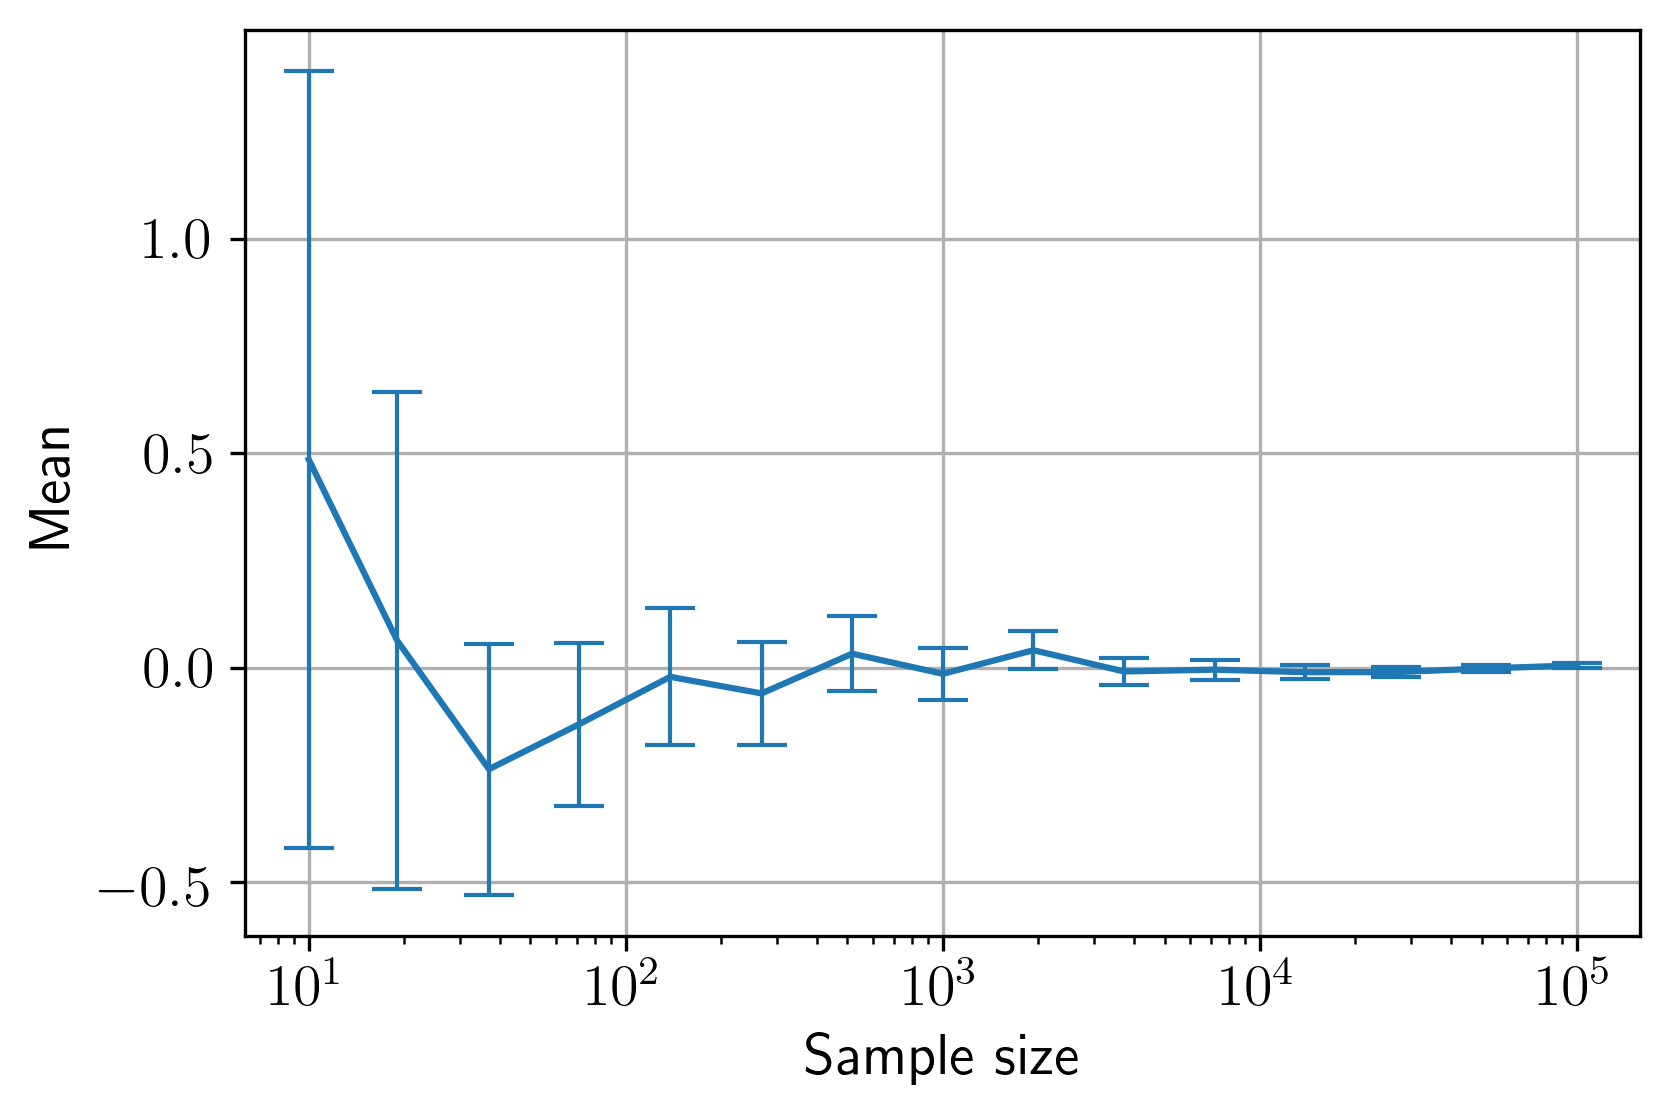
\includegraphics[width=0.5\textwidth]{figures/05_mean.png}
        \caption{Доверительные интервалы для математического ожидания.}
        \label{fig:05_mean}
    \hfill 
        \centering
        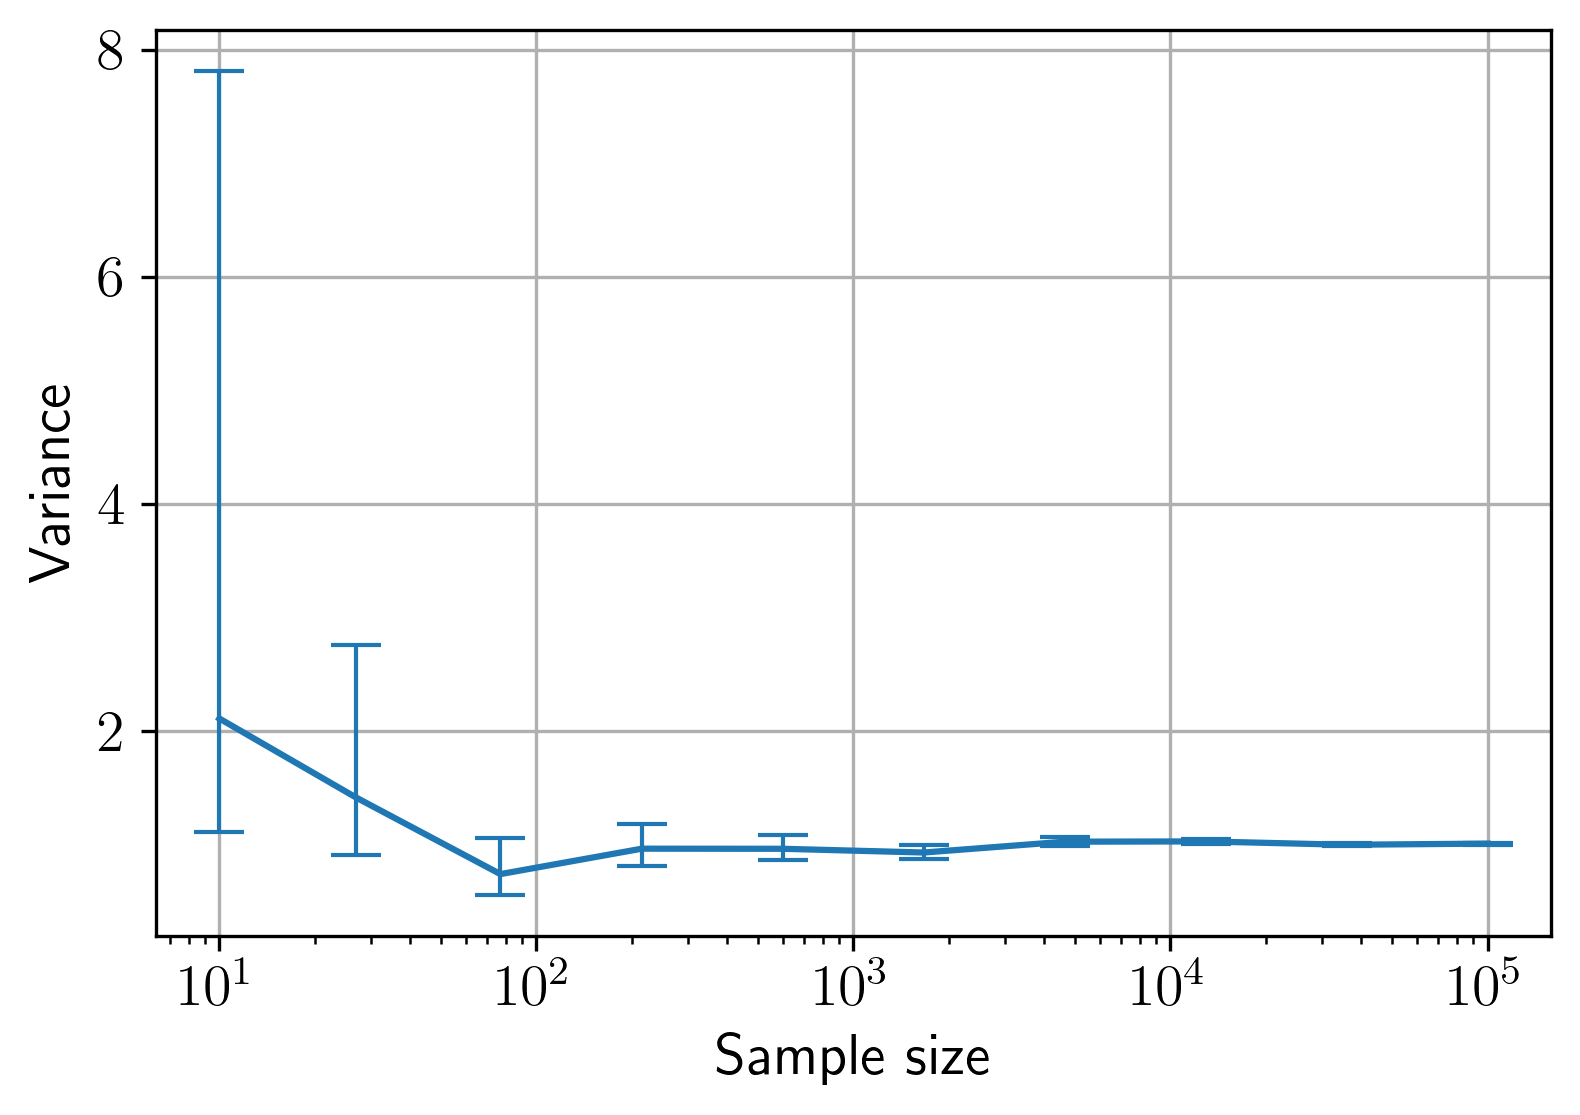
\includegraphics[width=0.5\textwidth]{figures/05_var.png}
        \caption{Доверительные интервалы для дисперсии.}
        \label{fig:05_var}
\end{multicols}
\end{figure}

Следующие 2 графика иллюстрируют поведение выборочных средних для распределения Коши.
На рис.~\ref{fig:05_cmeans} показано типичное поведение выборочного среднего в зависимости от числа элементов выборки.
На рис.~\ref{fig:05_cqq} нанесен Q-Q plot для квантилей выборки и теоретических квантилей распределения Коши.

\begin{figure}[H]
\begin{multicols}{2}
        \centering
        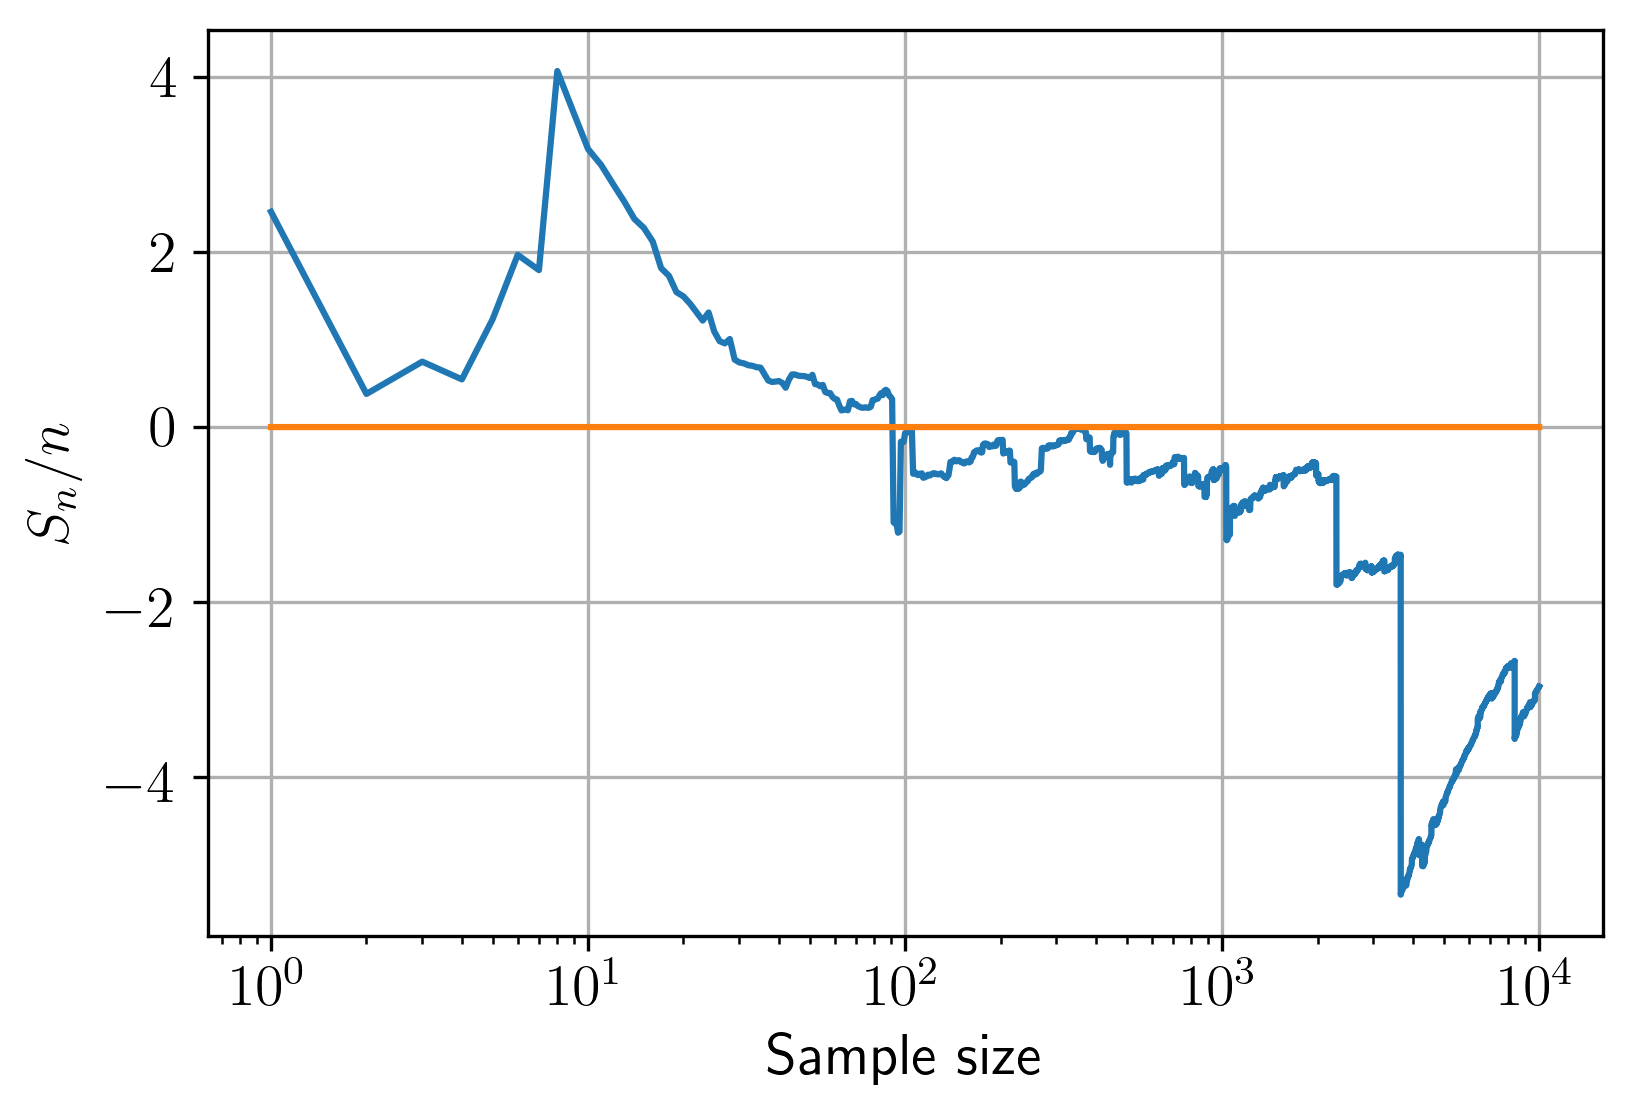
\includegraphics[width=0.5\textwidth]{figures/05_cmeans.png}
        \caption{Выборочное среднее $S_n / n$ в зависимости от $n$.}
        \label{fig:05_cmeans}
    \hfill 
        \centering
        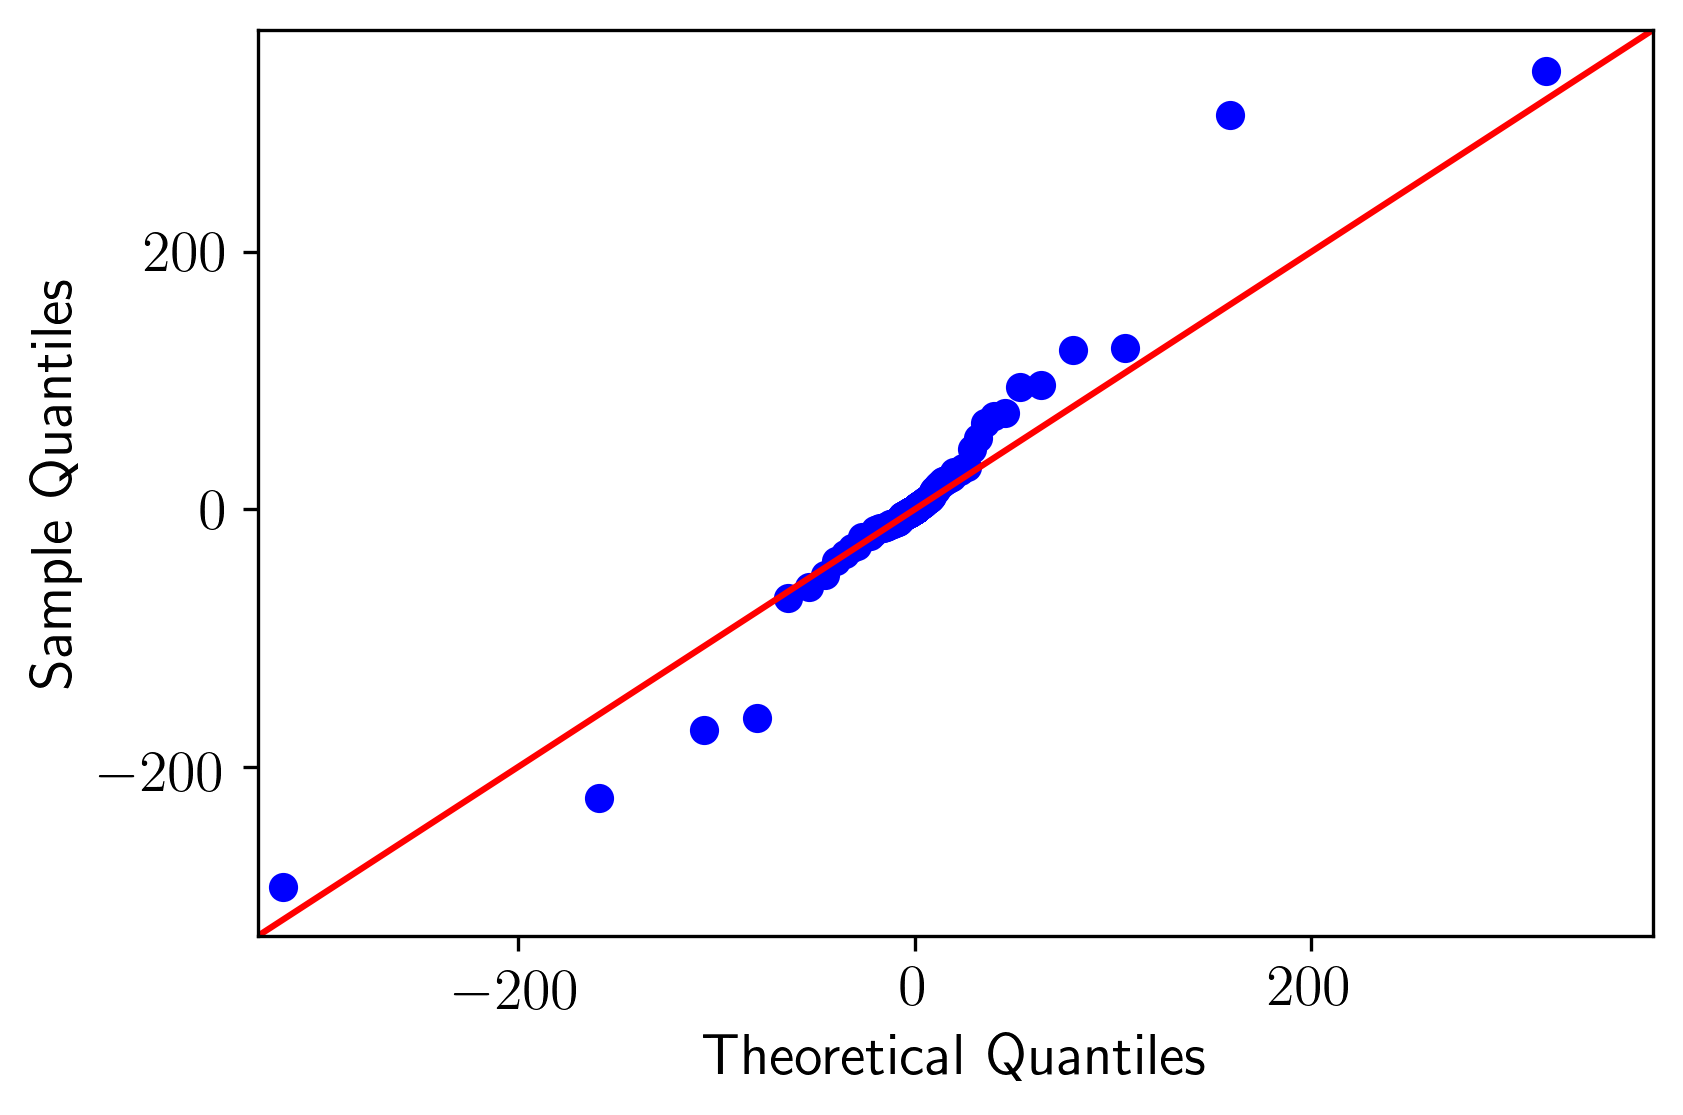
\includegraphics[width=0.5\textwidth]{figures/05_cqq.png}
        \caption{Распределение выборочного среднего. 1000 выборок по 1000 испытаний. Q-Q plot для распределения Коши.}
        \label{fig:05_cqq}
\end{multicols}
\end{figure}

\section{Задание 6}
\subsection{Постановка задачи}
\begin{enumerate}
\item Посчитать интеграл
$$J = \int\limits_{-\infty}^{+\infty}\int\limits_{-\infty}^{+\infty}\ldots\int\limits_{-\infty}^{+\infty} \dfrac{e^{-\left(x_1^2 + \ldots + x_{10}^2 + \frac{1}{2^7x_1^2\ldots x_{10}^2}\right)}}{x_1^2\ldots x_{10}^2}dx_1dx_2\ldots dx_{10}$$
\begin{itemize}
	\item методом Монте--Карло;
	\item методом квадратур, сводя задачу к вычислению собственного интеграла Римана.
\end{itemize} 
\item Для каждого случая оценить точность вычислений.
\end{enumerate}

\subsection{Теоретическая часть}

Рассмотрим вычисление интеграла методом Монте-Карло.
Положим 
\[
    g(\vec{x}) = \pi^{5} \frac{\exp \left\{ -\frac{1}{128 x_1^2 \ldots x_{10}^2} \right\}}{x_1^2 \ldots  x_{10}^2}.
\] 
Тогда интеграл можно записать в виде:
\[
    J = \Expec g(\vec{X}), 
\]
где $\vec{X}$ имеет 10-мерное нормальное распределение с нулевым средним и ковариационной матрицей $\frac{1}{2} I$.
Данное математическое ожидание будем вычислять как выборочное среднее 
$\hat{J} = \frac{1}{n} \sum\limits_{i=1}^{n} g(\vec{X_i})$.

Так как вычислить распределение $g(\vec{X})$ не представляется возможным, 
для оценки точности метода Монте-Карло будем использовать неравенство Чебышева:
\[
\Prob\left( \left\lvert J - \hat{J} \right\rvert \ge \epsilon \right) 
\le \frac{\var g(\vec{X_i})}{n\epsilon^2} = 1 - \alpha.
\]
Дисперсию будем аппроксимировать несмещенной оценкой:
$$\hat{\sigma}^2 = \frac{1}{n} \sum\limits_{i=1}^{n} \left( g(\vec{X_i}) - \overline{g(\vec{X_i})} \right)^2.$$
Тогда выражение для точности:
 \[
     \epsilon = \frac{\hat{\sigma}}{\sqrt{n(1 - \alpha)}}.
\] 

Для вычисления интеграла методом квадратур сделаем замену:
$$x_k = \tg\left(y_k\right), \quad dx_k = \dfrac{dy_k}{\cos^2\left(y_k\right)}, \ k = 1, \ldots, 10.$$
Тогда интеграл принимает вид:
$$\int\limits_{-\frac{\pi}{2}}^{\frac{\pi}{2}}\ldots\int\limits_{-\frac{\pi}{2}}^{\frac{\pi}{2}} \exp \left\{-\sum\limits_{k=1}^{10} \tg^2(y_k) - \dfrac{1}{128}\prod\limits_{k=1}^{10} \ctg^2 (y_k)\right\}\prod\limits_{k=1}^{10} \dfrac{1}{\sin^2(y_k)}dy_1\ldots dy_{10}$$
Данный интеграл является собственным и может быть вычислен методом квадратур.
Заметим, что функция является четной по каждой переменной, поэтому достаточно вычислить значение интеграла в положительном ортанте, а затем результат умножить на $2^{10}$.
Так же функция значение функции не меняется от перестановки переменных, поэтому для вычисления интеграла достаточно упорядочить элементы равномерной сетки в лексикографическом порядке,
затем каждую точку взять с весом 
\[
    \frac{10!}{r_1! \ldots r_{n}!},
\]
где $r_i$~---~число раз, которое повторяется  $i$-й по порядку элемент сетки в текущем наборе из 10 точек. 
Для численной устойчивости рекомендуется вычислять $n! / m!$ как $\exp\left\{\ln \Gamma (1 + n) - \ln \Gamma (1 + m)\right\}$. 

Для оценки погрешности будем использовать разложение в ряд Тейлора с остаточным членом в форме Лагранжа функции $g$:
$$g(y) = g(y_0) + \langle \nabla g(\xi), \ \Delta y\rangle,$$
где $y_0$ центр гиперкуба $\Delta$, a $\xi \in \Delta$. Интегрируя обе части по $\Delta$, получим, что ошибка интегрирования по каждому гиперкубу равна
$$\int\limits_\Delta \langle \nabla g(\xi), \ \Delta y\rangle dy \leq \sup_\Delta \|\nabla g(x)\|\cdot\|\Delta y\|\cdot\mu(\Delta) \leq \dfrac{\sqrt{n}}{2}h^{n+1}\sup_{\left[-\frac{\pi}2, \frac{\pi}2\right]} \|\nabla g(x)\|,$$
а общая ошибка не превосходит $\dfrac{\pi^nh\sqrt{n}}{2}\sup\limits_{\left[-\frac{\pi}2, \frac{\pi}2\right]} \|\nabla f(x)\|$.
Однако даже при вычислении 10-мерного интеграла шаг сетки получается таким малым, что вычисление с таким шагом не представляется возможным.
\subsection{Результаты работы программы}

При вычислении интеграла методом Монте-Карло был получен результат $\hat{J} = 124{,}83$, и оценка погрешности $\epsilon = 0{,}05$. Число испытаний $10^{10}$.
Методом квадратур был полуен результат $J \approx 124{,}81$ на сетке размером 30 по каждому измерению.

\section{Задание 7}
\subsection{Постановка задачи}
\begin{enumerate}
	\item Методом случайного поиска найти минимальное значение функции $f$ на множестве $$A = \left\{(x_1, x_2)\colon \ x_1^2 + x_2^2 \leq 1\right\},$$ где 
 $$f(x_1, x_2) = x_1^3\sin\left(\dfrac{1}{x_1}\right) + 10x_1x_2^4 \cos\left(\dfrac{1}{x_2}\right),$$
 $f(0, 0) = 0$ по непрерывности.
	\item Методом имитации отжига найти минимальное значение функции Розенброка $g$ в пространстве $\mathbb{R}^2$, где
$$g(x) = (x_1 - 1)^2 + 100(x_2 - x_1^2)^2.$$
	\item Оценить точность. Сравнить результаты со стандартными методами оптимизации.
\end{enumerate}
\subsection{Теоретическая часть}

Для поиска минимума функции методом случайного поиска будем генерировать 
независимые равномерно распределенные в $A$ случайные  величины.
Затем в полученной выборке найдем ту реализацию, на которой значение функции минимально. 

Для генериорвания равномерного распределения в круге найдем распределение полярных координат равномерно распределенных точек:
\[
    \mathbb{P}(X \in M) = \dfrac{1}{\pi}\iint\limits_Mdxdy = \dfrac{1}{\pi}\iint\limits_Mr\,drd\varphi = \iint\limits_Mdr^2\,d\left(\dfrac{\varphi}{2\pi}\right).
\] 
Отсюда следует, что радиус и угол независимы, угол распределен равномерно, а функция распределения радиуса имеет вид:
\[
    F_r(x) = x^2\left[ 0 \le x \le 1 \right].
\] 
Таким образом, случайная величина $X$ с полярными координатами  $(r, \phi)$
будет распределена равномерно в  $A$, если  $\phi \sim U[0, 2\pi]$ и 
$\Pro(r < x) = F_r(x)$. 

Оценим точность для метода случайного поиска. 
Потребуем, чтобы $|f(x) - f(x^*)| < \varepsilon$:
$$
|f(x) - f(x^*)| \leqslant \| \nabla f(x^*) \| \cdot\|x - x^*\| \leqslant
\max\limits_{\| x \| \leqslant 1} \| \nabla f(x) \| \cdot \| x - x^* \| =
\max\limits_{\| x \| \leqslant 1} \| \nabla f(x) \| \delta
$$
Оценим норму градиента:
\[
\frac{\partial f}{\partial x_1} = 3x_1^2\sin\left(\frac{1}{x_1}\right) - x_1\cos\left(\frac{1}{x_1}\right) + 10x_2^4\cos\left(\frac{1}{x_2}\right),
\]
\[
\frac{\partial f}{\partial x_2} = 40x_1x_2^3 \cos\left(\frac{1}{x_2}\right) + 10x_1x_2^2\sin\left(\frac{1}{x_2}\right).
\]
Тригонометрический функции и переменные оценим сверху по модулю числом $1$. Тогда:
$$
\max\limits_{\| x \| \leqslant 1} \| \nabla f(x) \| \leqslant
\sqrt{14^2 + 50^2} \leqslant 52
$$
Таким образом
$$
\delta = \frac{\varepsilon}{52}
$$

Потребуем, чтобы с вероятностью не менее $\alpha$ хотя бы одна точка выборки попала в $\delta$-окрестность точки минимума.
Эквивалентно: с вероятностью не превосходящей $1 - \alpha$ ни одна точка не должна попасть в $\delta$-окрестность искомой точки. Так как требуется получить верхнюю оценку, то, чтобы не учитывать границы, заменим окружность с радиусом $\delta$ на полуокружность:
$$
\mathbb{P}\bigl( \forall x \in \mathbb{X} \colon x \notin B_\delta(x^*) \bigr) \leqslant 
\left( \frac{\pi - \pi \delta^2/2}{\pi} \right)^n = \left( 1 - \delta^2/2 \right)^n 
\leqslant 1 - \alpha.
$$
Отсюда 
$$
\varepsilon = 52\delta = 52\sqrt{2 - 2\sqrt[n]{1 - \alpha}}
$$

Описание метода имитации отжига:
\begin{enumerate}
    \item Задается функция для минимизации $f(\cdot)$ начальная температура $T_0$, начальное приближение $x_0$,
        распределение шага по переменной $\mathcal{P}$ и функцию понижения температуры $h(\cdot)$.
    \item На каждой итерации цикла вычисляется следующее положение точки $x' = x_i + \xi$, где $\xi \sim \mathcal{P}$.
    \item Если $f(x') < f(x_i)$, то $x_{i+1} = x'$, иначе $x_{i+1} = x'$ с вероятностью $p_i = \exp \left\{ \frac{f(x_i) - f(x')}{T_i} \right\}$
        и $x_{i+1} = x_i$ с вероятностью $1 - p_i$.
    \item Понижается температура  $T_{i+1} = h(T_i)$.
\end{enumerate} 

\subsection{Результаты работы программы}
В резуьтате работы программы для первой части задания была найдена точка минимума $(-0{,}367, 0{,}930)$.
Размер выборки  $10^6$, точность  $0{,}13$ с надежностью  $0{,}95$.

Для функции Розенброка методом имитации отжига был найден минимум  $(1{,}003, 1{,}005)$.
Было проведено  16111 итераций и 1642 раза была обновлена точка. 
В качестве распределения для шага было выбрано нормальное распределение с нулевым средним и стандартным отклонением  $0{,}05$.
НАчальное приближение~--- точка  $(0, 0)$, 
температура понижалась по закону  $T = T_0 k^i$, где  $T_0 =1$,  $k = 0{,}999$, а $i$~--- номер итерации.

Стандартные методы нелинейной оптимизации в \texttt{scipy} лучше отработали на функции Розенброка, 
но не справились с первой функцией из-за большого количества локальных экстремумов, расположенных крайне нерегулярно.

\section{Задание 8}
\subsection{Постановка задачи}
\begin{enumerate}
	\item Применить метод Монте--Карло к решению первой краевой задачи для двумерного уравнения Лапласа в единичном круге:
$$
\begin{cases}
\Delta u = 0, \quad (x, y) \in D = \{(x, y)\colon \ \ x^2 + y^2 \le 1\}\\
u|_{\partial D} = f(x, y) \\
u \in C^2(D), \ f \in C(\partial D)
\end{cases}
$$

Для функции $f(x, y) = x^2 - y^2$ найти аналитическое решение и сравнить с полученным по методу Монте--Карло.
\end{enumerate}

\subsection{Теоретическая часть}
Кратко опишем способ решения данной задачи, полное описание можно найти в~\cite{Buslenko}.
Введем на плоскости равномерную сетку с шагом $h$ и назовем внутренними узлы, для которых все 4 соседних узла лежат в круге. 
Узлы, лежащие в круге, но не удовлетворяющие этому условию, будем называть крайними. 

Аппроксимируя вторые частные производные, можно свести задачу Дирихле к следующей разностной схеме:
$$u_{ij} = \dfrac14(u_{i-1,j} + u_{i+1, j} + u_{i, j-1} + u_{i,j+1})$$
для внутренних узлов, и
$$u_{ij} = f_{ij}$$
для крайних узлов.

Рассмотрим теперь следующую модель случайного блуждания: 
\begin{itemize}
	\item Частица начинает свой путь в одном из внутренних узлов $x_{ij}$.
	\item С равными вероятностями она переходит в один из четырех соседних узлов, пока частица не попадет на крайний узел $x_{pq}$.
\end{itemize}


Обозначим $p(x_{ij}, x_{pq})$ вероятность, начав путь в узле $x_{ij}$, закончить его в узле $x_{pq}$. Из формулы полной вероятности следует
\begin{equation}\label{Dirich}
p(x_{ij}, x_{pq}) = \dfrac14\bigl(p(x_{i-1,j}, x_{pq}) + p(x_{i+1, j}, x_{pq}) + p(x_{i, j-1}, x_{pq}) + p(x_{i,j+1}, x_{pq})\bigr)
\end{equation}
для внутренних узлов $x_{ij}$ и $p(x_{ij}, x_{ij}) = 1$ для крайних узлов.

Рассмотрим теперь случайную величину $\xi_{ij} = f(x_{pq})$ --- значение $f$ в конечной точке пути.
Так как $\mathbb{E}\xi_{ij} = \sum_{p, q}p(x_{ij}, x_{pq})f(x_{pq})$, используя формулу (\ref{Dirich}) связи вероятностей на соседних узлах, получим
$$\mathbb{E}\xi_{ij} = \dfrac14(\mathbb{E}\xi_{i-1,j} + \mathbb{E}\xi_{i+1, j} + \mathbb{E}\xi_{i, j-1} + \mathbb{E}\xi_{i,j+1}) \text{ для внутренних узлов,}$$
$$\mathbb{E}\xi_{ij} = f_{ij} \text{ для крайних}.$$

Видно, что эти уравнения совпадают с разностной схемой, аппроксимирующей исходную задачу.

Значения $\mathbb{E}\xi_{ij}$ в каждом узле можно вычислить методом Монте--Карло, моделируя описанный выше случайных процесс. 

Для оптимизации вычислений воспользуемся тем, что моделируемый процесс случайного блуждания обладает марковским свойством, поэтому при прохождении траектории через промежуточные узлы дальнейший путь частицы можно рассматривать как процесс, начавшийся в этом промежуточном узле.

Точным решением данной задачи является функция $f(x, y) = x^2 - y^2$.

\subsection{Результаты работы программы}

\begin{figure}[H]
    \centering
    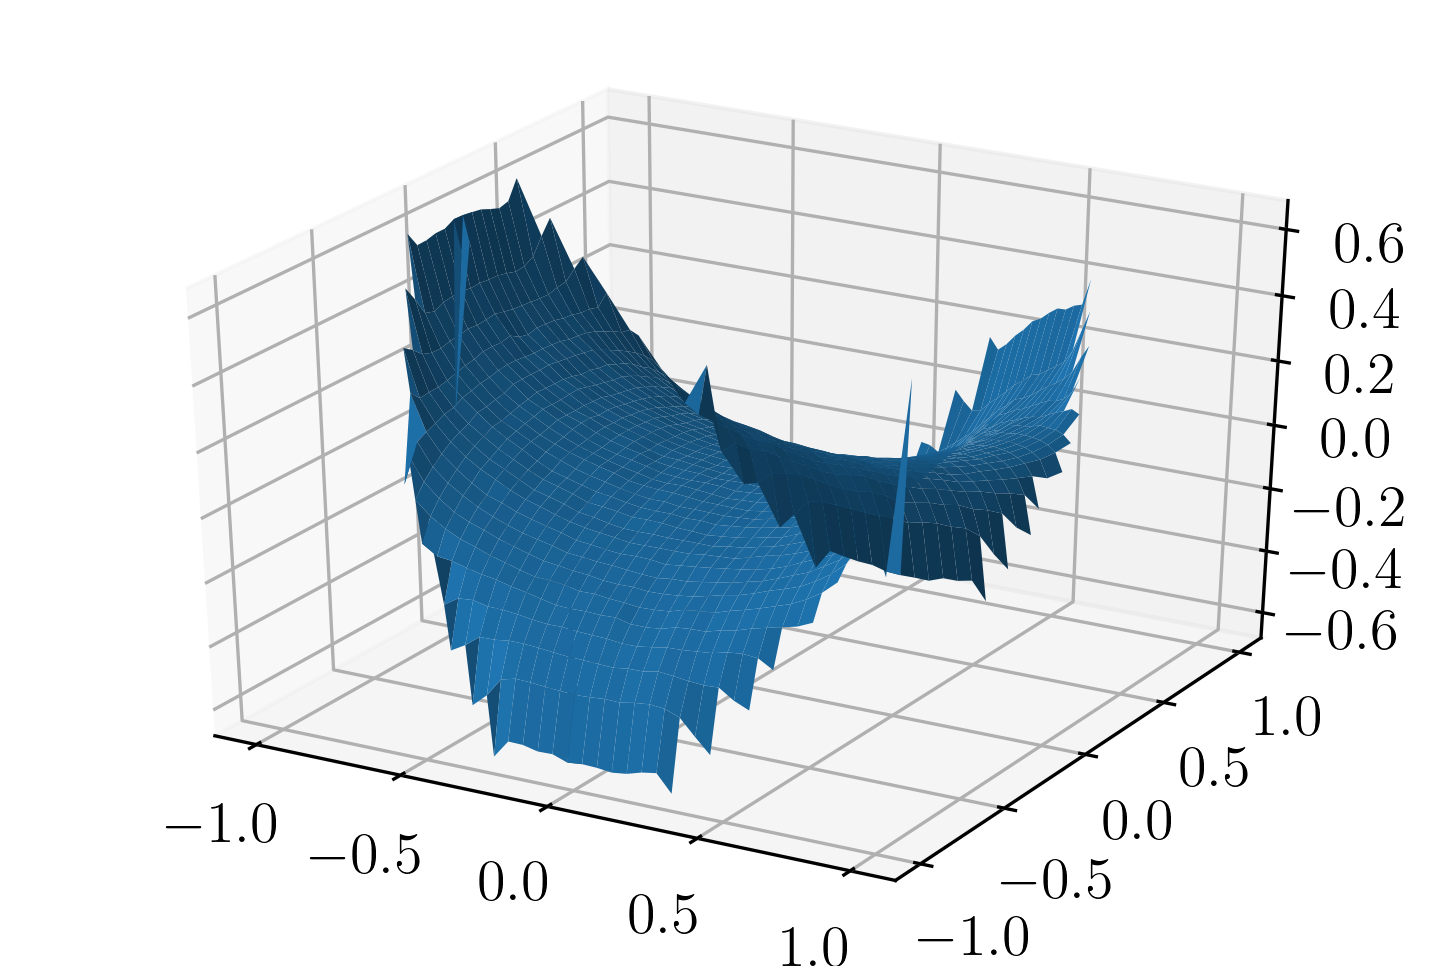
\includegraphics[width=0.5\textwidth]{figures/08_mc.png}
    \caption{Численное решение.}
    \label{fig:08_mc}
\end{figure}
\begin{figure}[H]
    \centering
    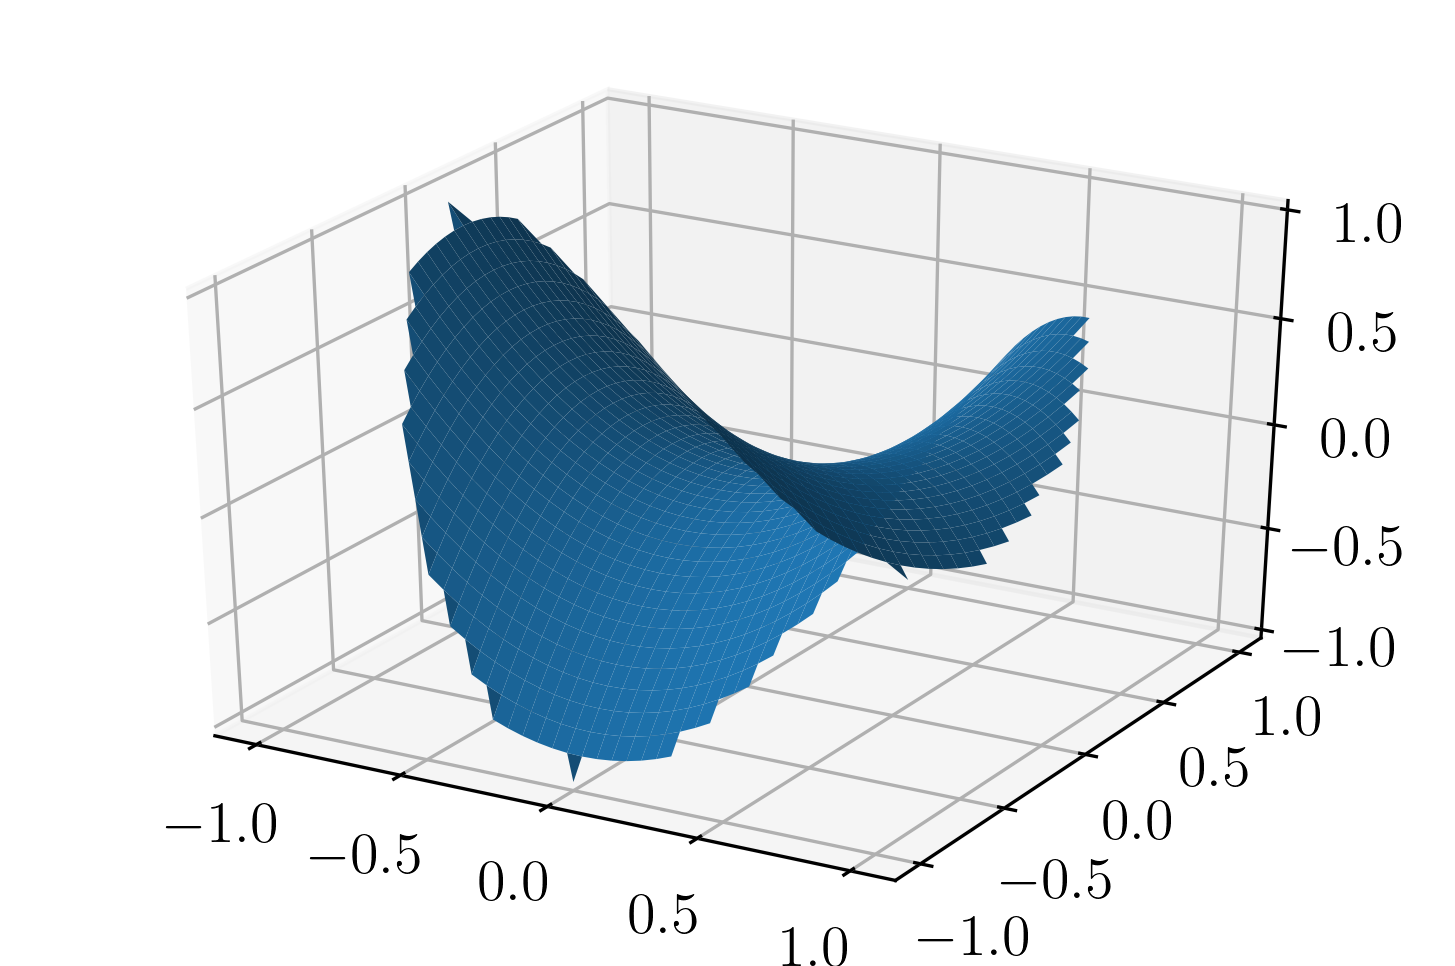
\includegraphics[width=0.5\textwidth]{figures/08_anal.png}
    \caption{Аналитическое решение.}
    \label{fig:08_anal}
\end{figure}
\begin{figure}[H]
    \centering
    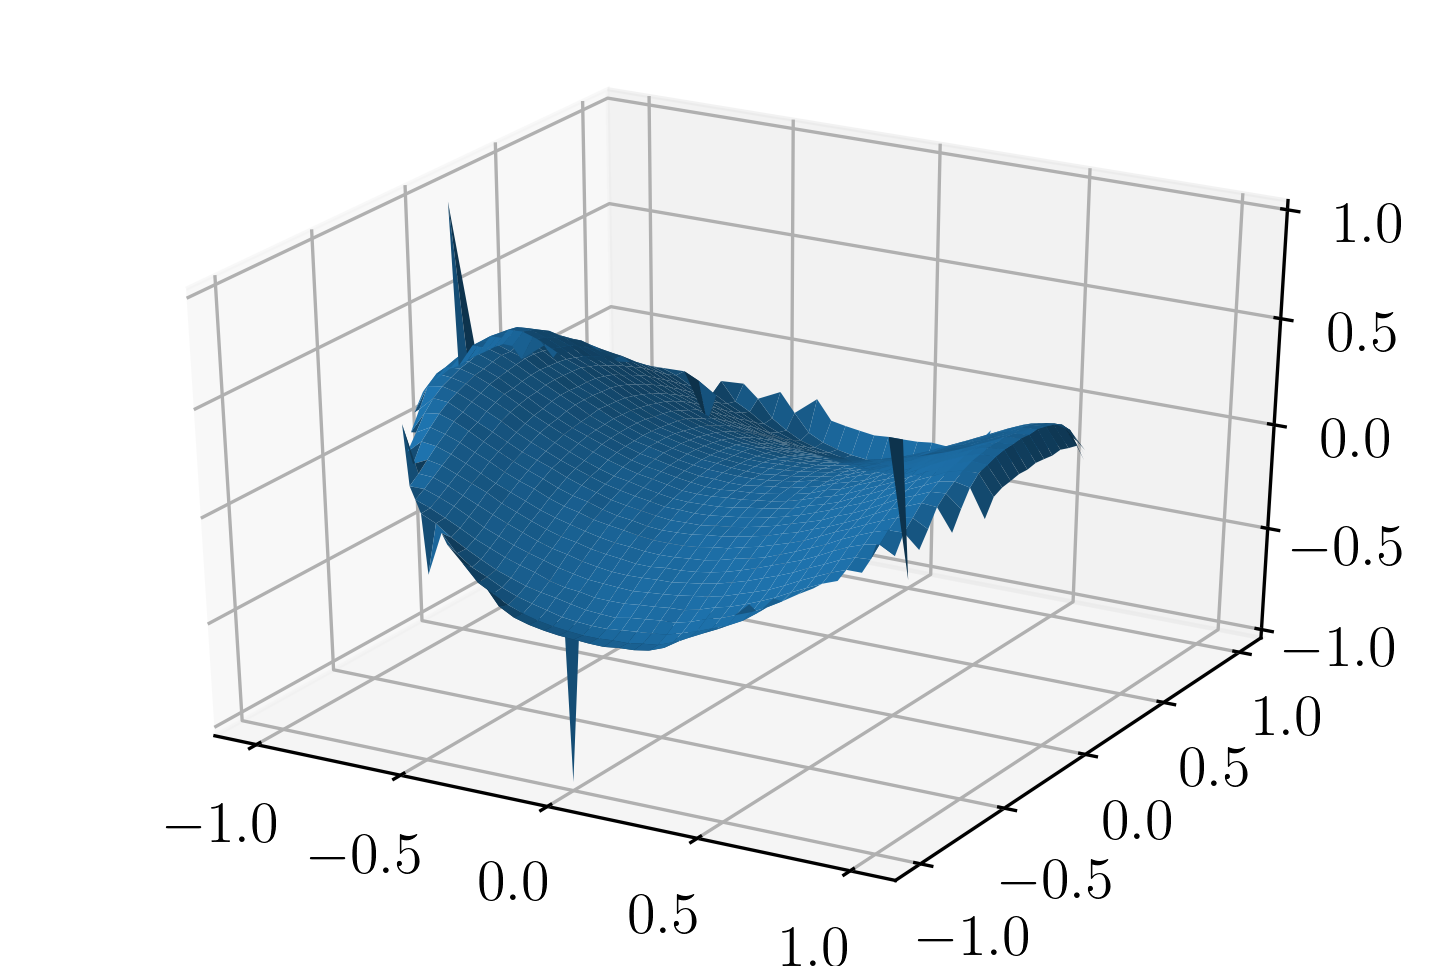
\includegraphics[width=0.5\textwidth]{figures/08_discr.png}
    \caption{Невязка}
    \label{fig:08_discr}
\end{figure}

\section{Задание 9}
\subsection{Постановка задачи}
Рассмотреть два вида процессов:
\begin{itemize}
	\item Винеровский процесс $W(t), t \in [0, 1], \ W(0) = 0.$
	\item Процесс Орнштейна--Уленбека $X(t),\ t \in [0, 1], \ X(0) = X_0$, то есть стационарный марковский гауссовский процесс. Начальное значение $X_0$ генерируется случайным образом так, чтобы полученный процесс бы стационарным.
\end{itemize}

Для данных процессов
\begin{enumerate}
	\item Найти ковариационную функцию и переходные вероятности.
	\item Промоделировать независимые траектории процесса с данными переходными вероятностями методом добавления разбиения отрезка.
	\item Построить график траекторий, не соединяя точки ломаной с целью получения визуально непрерывной линии.
\end{enumerate}

\subsection{Теоретическая часть}
Опишем метод разбиения отрезка для моделирования случайного процесса.
\begin{enumerate}
    \item Сгенерировать $X(0)$.
    \item Сгенерировать  $X(1) \sim \Pro\bigl(X(1) \mid X(0)\bigr)$ 
    \item Пусть случайный процесс уже сгенерирован в точках  $t_1$ и $t_3$.
        Тогда $X(t_2) \sim \Pro\bigl( X(t_2) \mid X(t_1), X(t_3) \bigr)$.
    \item Повторять, пока разбиение не получится достаточно мелким.
\end{enumerate} 

Найдем выражение для условных вероятностей Винеровского процесса.
Пусть $t > s$, тогда
\begin{multline*}
    k(t, s) = \mathbb{E}[W(t)W(s)] = \mathbb{E}\left[W(s)^2\right] + \mathbb{E}\left[W(s)(W(t) - W(s))\right] =  \\ =
    \mathbb{E}\left[W(s)^2\right] + \mathbb{E}\left[W(s)\right]\mathbb{E}\left[(W(t) - W(s))\right] = 
    \sigma^2 \min(t, s)
\end{multline*}

Для метода деления отрезка пополам найдем условное распределение $\mathbb{P}\bigl(W(t) = x_2 \mid W(t - \Delta t) = x_1, W(t + \Delta t) = x_3\bigr)$.
По теореме Байеса и определению условной плотности имеем:
\begin{multline*}
    p\bigl(W(t) = x_2 \mid W(t - \Delta t) = x_1, W(t + \Delta t) = x_3\bigr) = \\ =
    \frac{p\bigl(W(t + \Delta t) = x_3 | W(t) = x_2\bigr) p\bigl(W(t) = x_2 | W(t - \Delta t) = x_1\bigr)}{p\bigl(W(t + \Delta t) = x_3 | W(t - \Delta t) = x_1\bigr)} =\\
    =\frac{\mathcal{N}(x_3 | x_2, \Delta t \sigma^2)\mathcal{N}(x_2 | x_1, \Delta t \sigma^2)}{\mathcal{N}(x_3 | x_1, 2 \Delta t \sigma^2)} = \mathcal{N}\left(x_2 \biggm| \frac{x_1 + x_3}{2}, \frac{\Delta t \sigma^2}2\right).
\end{multline*}

Процесс Орнштейна-Уленбека - это стационарный марковский гауссовский процесс. Без ограничения общности рассмотрим центрированный процесс.
Для корреляционной функции такого процесса верны свойства:
$$
\rho(t_1, t_3)) = \rho(t_1, t_2)\rho(t_2, t_3), \quad t_1 < t_2 < t_3, \\
\rho(t, s) = \rho(|t - s|), \quad t < s.
$$
Отсюда $\rho(a + b) = \rho(a)\rho(b)$.
Учитвая то, что корреляционная функция ограничена, получаем, что
$$
\rho(t, s) = \sigma^2e^{-\lambda |t - s|}, \quad \lambda > 0.
$$

Аналогично по теореме Байеса и определению условной плотности имеем:
\begin{multline*}
    p\bigl(X(t) = x_2 \mid X(t - \Delta t) = x_1, X(t + \Delta t) = x_3\bigr) = \\ 
    =\mathcal{N}\left(\frac{x_1 + x_3}{2 \cosh (\lambda \Delta t)}, \sigma^2 \tanh (\lambda \Delta t) \right)
\end{multline*}

\subsection{Результаты работы программы}

Следующие графики были получены при моделировании стандартного Винеровского процесса и стандартного процесса Орнштейна--Уленбека.
Отрезок $[0, 1]$ был разбит на  $2^{12}$  частей.
\begin{figure}[H]
    \centering
    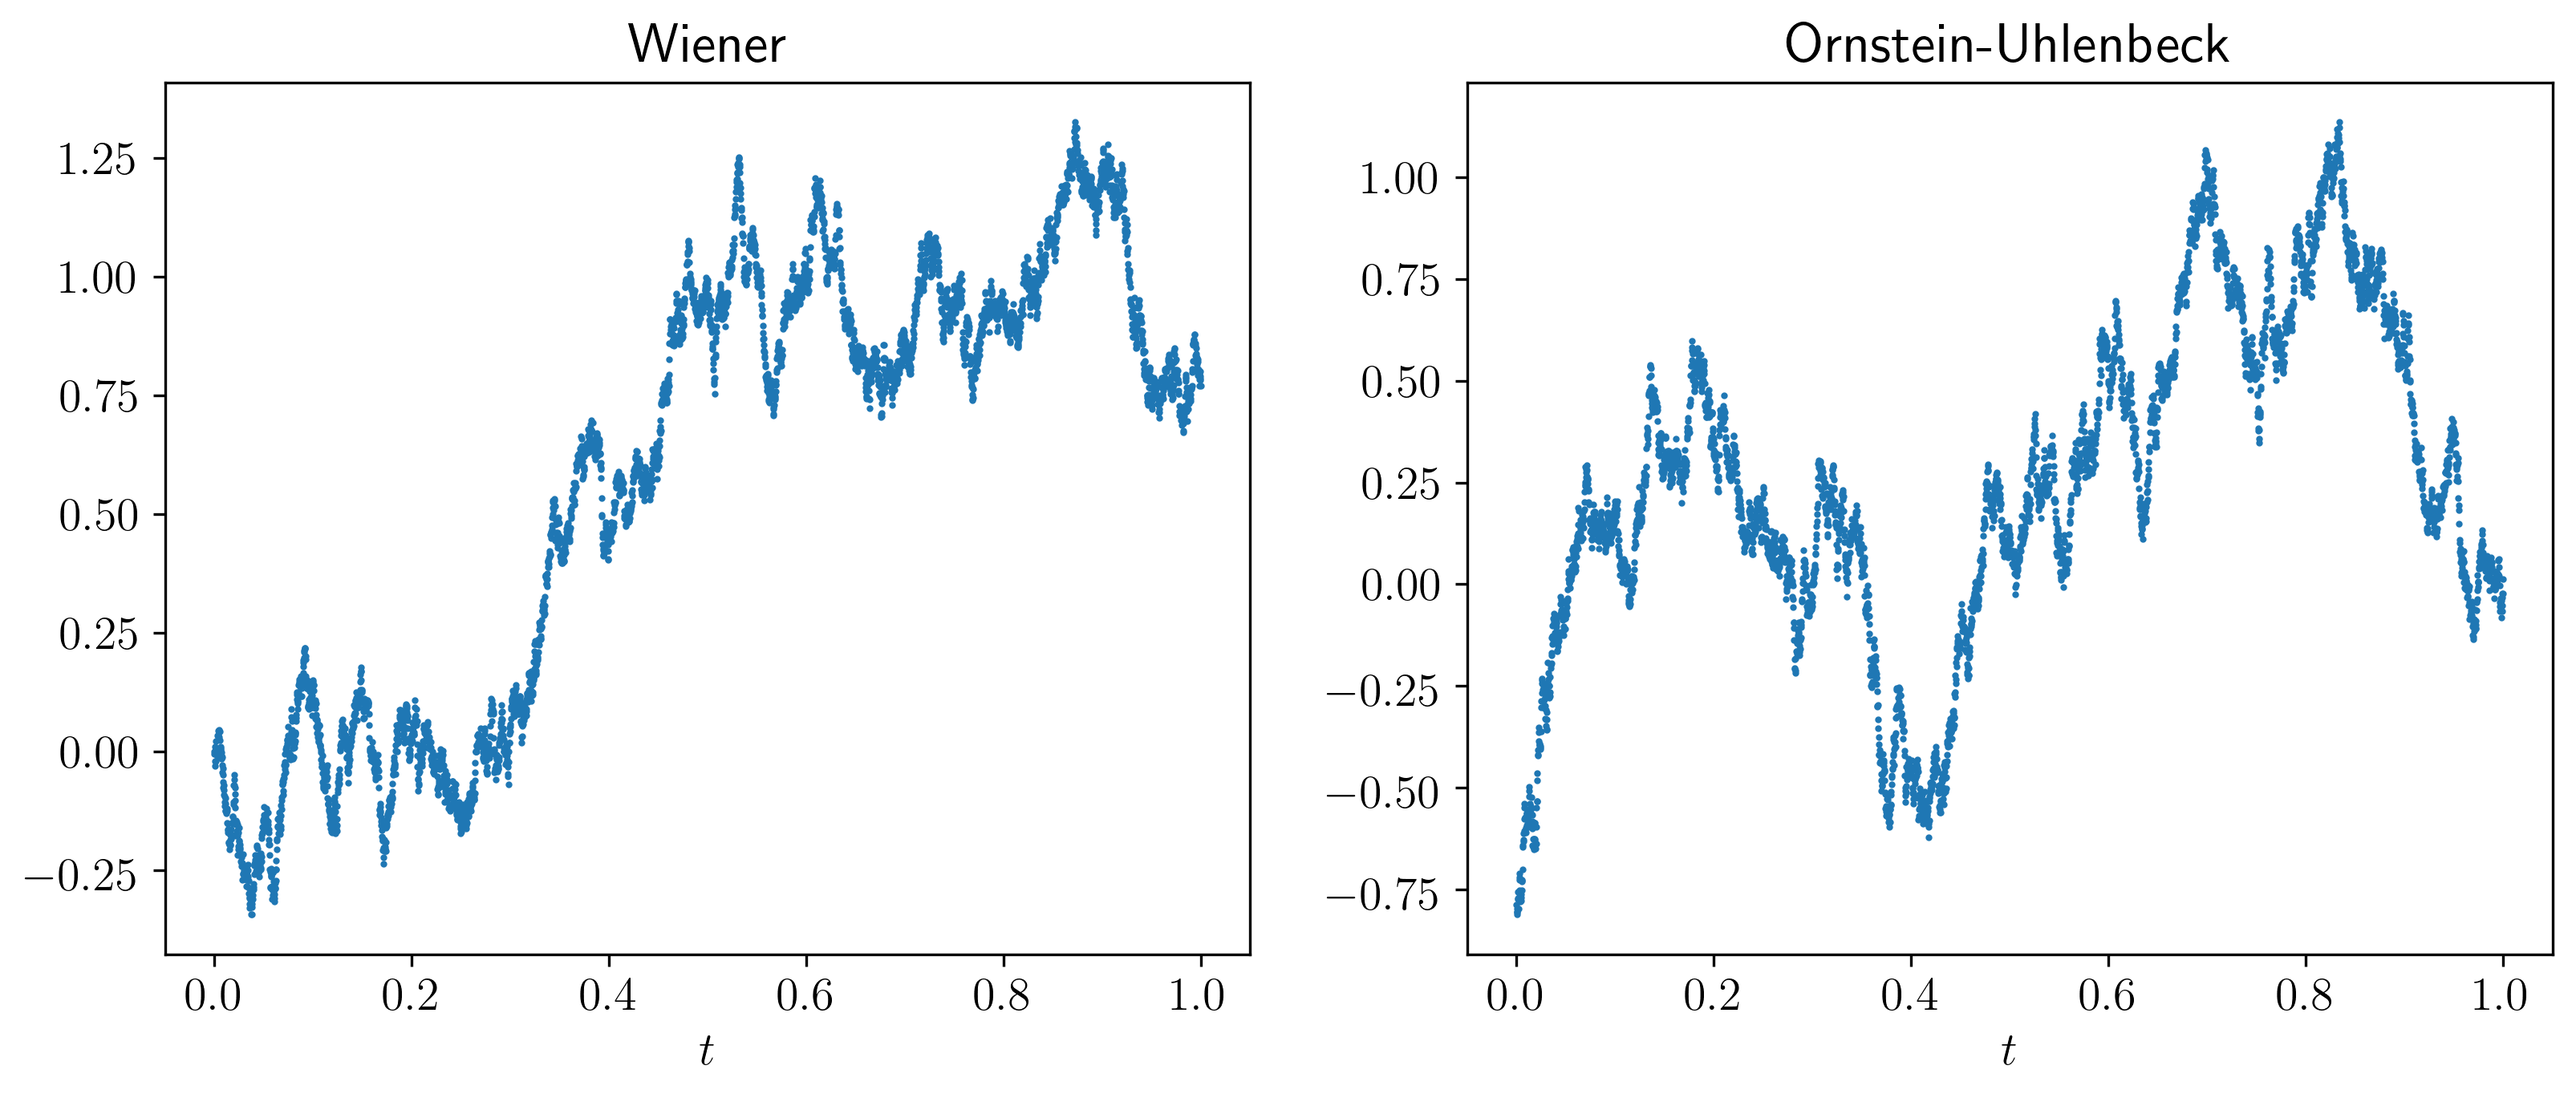
\includegraphics[width=\textwidth]{figures/09_proc.png}
    \caption{Траектории процессов.}
    \label{fig:09_proc}
\end{figure}

\section{Задание 10}
\subsection{Постановка задачи}
Произвести фильтрацию одномерного процесса Орнштейна--Уленбека:
\begin{enumerate}
	\item Используя генератор белого шума, добавить случайную ошибку с известной дисперсией к реализации процесса Орнштейна--Уленбека.
	\item При помощи одномерного фильтра Калмана оценить траекторию процесса по зашумленному сигналу. Параметры процесса и белого шума считать известными.
	\item Рассмотреть случай, когда шум
	\begin{itemize}
		\item является гауссовским;
		\item имеет распределение Коши.
	\end{itemize}
\end{enumerate}

\subsection{Теоретическая часть}
Рассмотрим процесс с дискретным временем $t_i = hn$, где $n = \overline{0,\ldots N}$.
Рассмотрим на этой сетке процесс Орнштейна--Уленбека со значениями  $x_n = X(t_n)$.
Для применения фильтра Калмана~\cite{Bishop} представим процесс в виде одномерной линейной системы:
\[
    \begin{cases}
        x_{n+1} = ax_n + \nu_n, \\
        \nu_n \sim \Norm(0, q), \\
        x_0 \sim \Norm(0, \sigma^2).
    \end{cases}
\] 
Мы можем наблюдать только зашумленный сигнал:
\[
    \begin{cases}
        y_n = x_n + \epsilon_n,\quad n = \overline{1,\ldots N}, \\
        \epsilon_n \sim \Norm(0, r), \\
        y_0 = x_0.
    \end{cases}
\] 

Обозначим за $\hat x_{n \mid n}$ оценку значения $x_n$ при известных $y_1, \ldots y_n$. $\hat x_{n \mid n-1}$~--- экстраполяция процесса на следующий шаг в соответствии с динамической системой.
Через $p_{n \mid n}$ будем обозначать дисперсию ошибки фильтрации на $n$-м шаге, через $p_{n\mid n-1}$ --- прогнозируемую на следующем шаге дисперсию.
Опишем один шаг дискретного фильра Калмана:
\begin{enumerate}
    \item Прогнозируем процесс и дисперсию на 1 шаг вперед:
        \[
            \begin{cases}
                \hat{x}_{n\mid n-1} = a \hat{x}_{n - 1\mid n-1}, \\
                p_{n \mid n - 1} = a^2 p_{n - 1 \mid n - 1} + q.
            \end{cases}
        \] 
    \item Вычисляем отклонение прогноза от шумного сигнала и коэффициент усиления Калмана:
        \[
            \begin{cases}
                \delta_n = y_n - \hat{x}_{n \mid n-1}, \\
                k_n = \frac{p_{n\mid n-1}}{p_{n \mid n-1} + r}.
            \end{cases} 
        \] 
    \item Фильруем шум и оцениваем ошибку:
        \[
            \begin{cases}
                \hat{x}_{n \mid n} = \hat{x}_{n \mid n-1} + k_n \delta_n,\\
                p_{n \mid n} = (1 - k_n) p_{n\mid n-1}.
            \end{cases} 
        \] 
\end{enumerate} 

Так как все распределения в данной процедуре являются гауссовскими, то и ошибка будет распределена нормально.
Отсюда можно выписать выражение для доверительного интервала с уровнем доверия $\alpha$:
 \[
     \Delta = \sqrt{p_{n\mid n}} \Phi^{-1}\left(\frac{1+\alpha}{2}\right). 
\] 

\subsection{Результаты работы программы}

\begin{figure}[H]
    \centering
    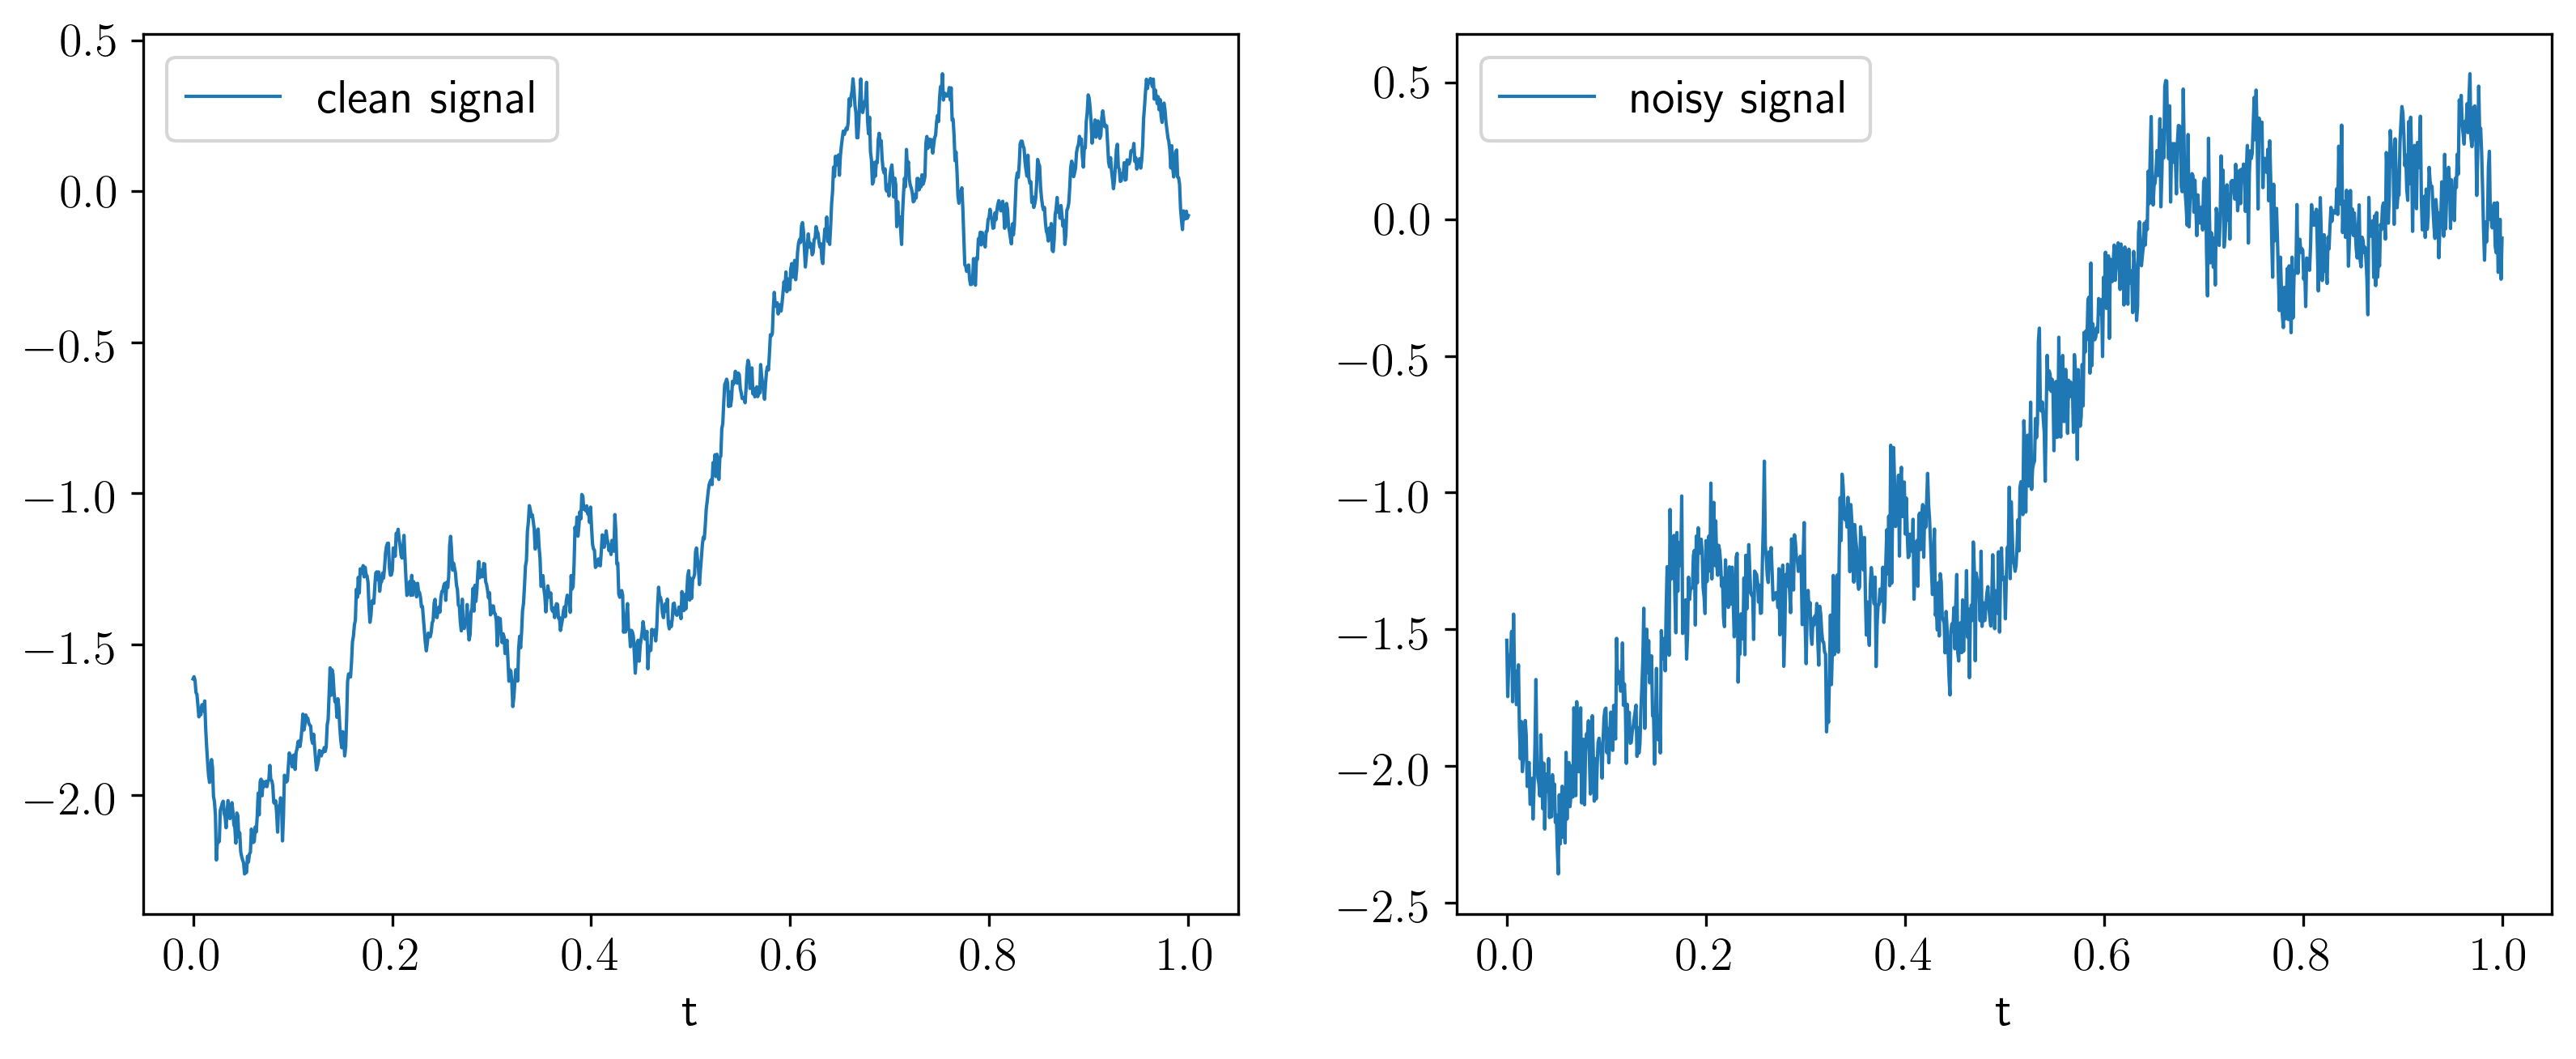
\includegraphics[width=\textwidth]{figures/10_noisy.png}
    \caption{Чистый и зашумленный гауссовским шумом сигналы, полученные с помощью стандартного процесса Орнштейна--Уленбека.}
    \label{fig:10_noisy}
\end{figure}
\begin{figure}[H]
    \centering
    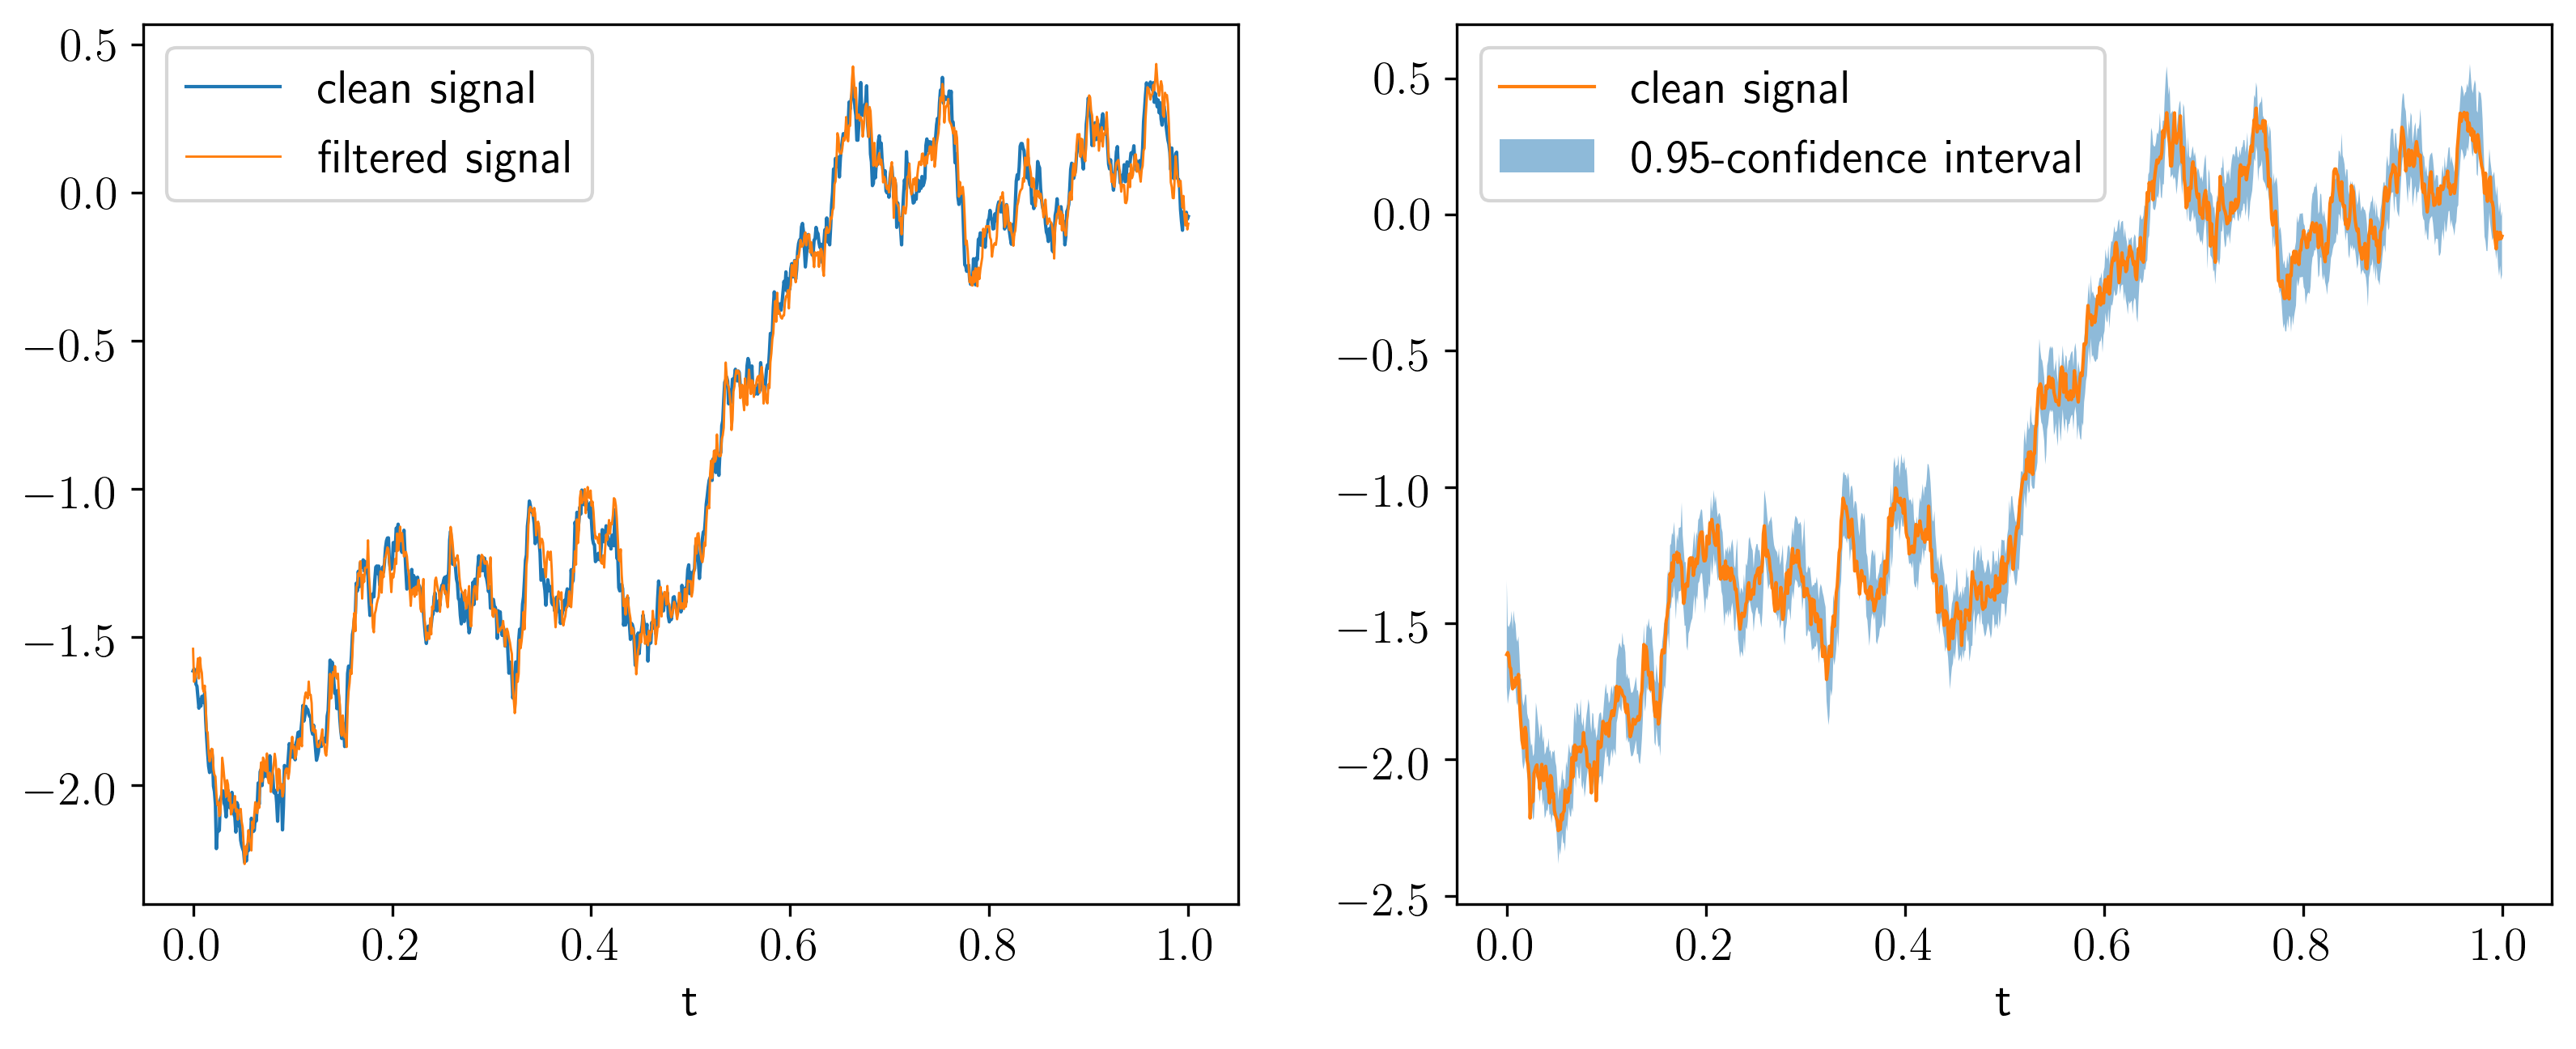
\includegraphics[width=\textwidth]{figures/10_filtered.png}
    \caption{Результаты фильтрации.}
    \label{fig:10_filtered}
\end{figure}
\begin{figure}[H]
    \centering
    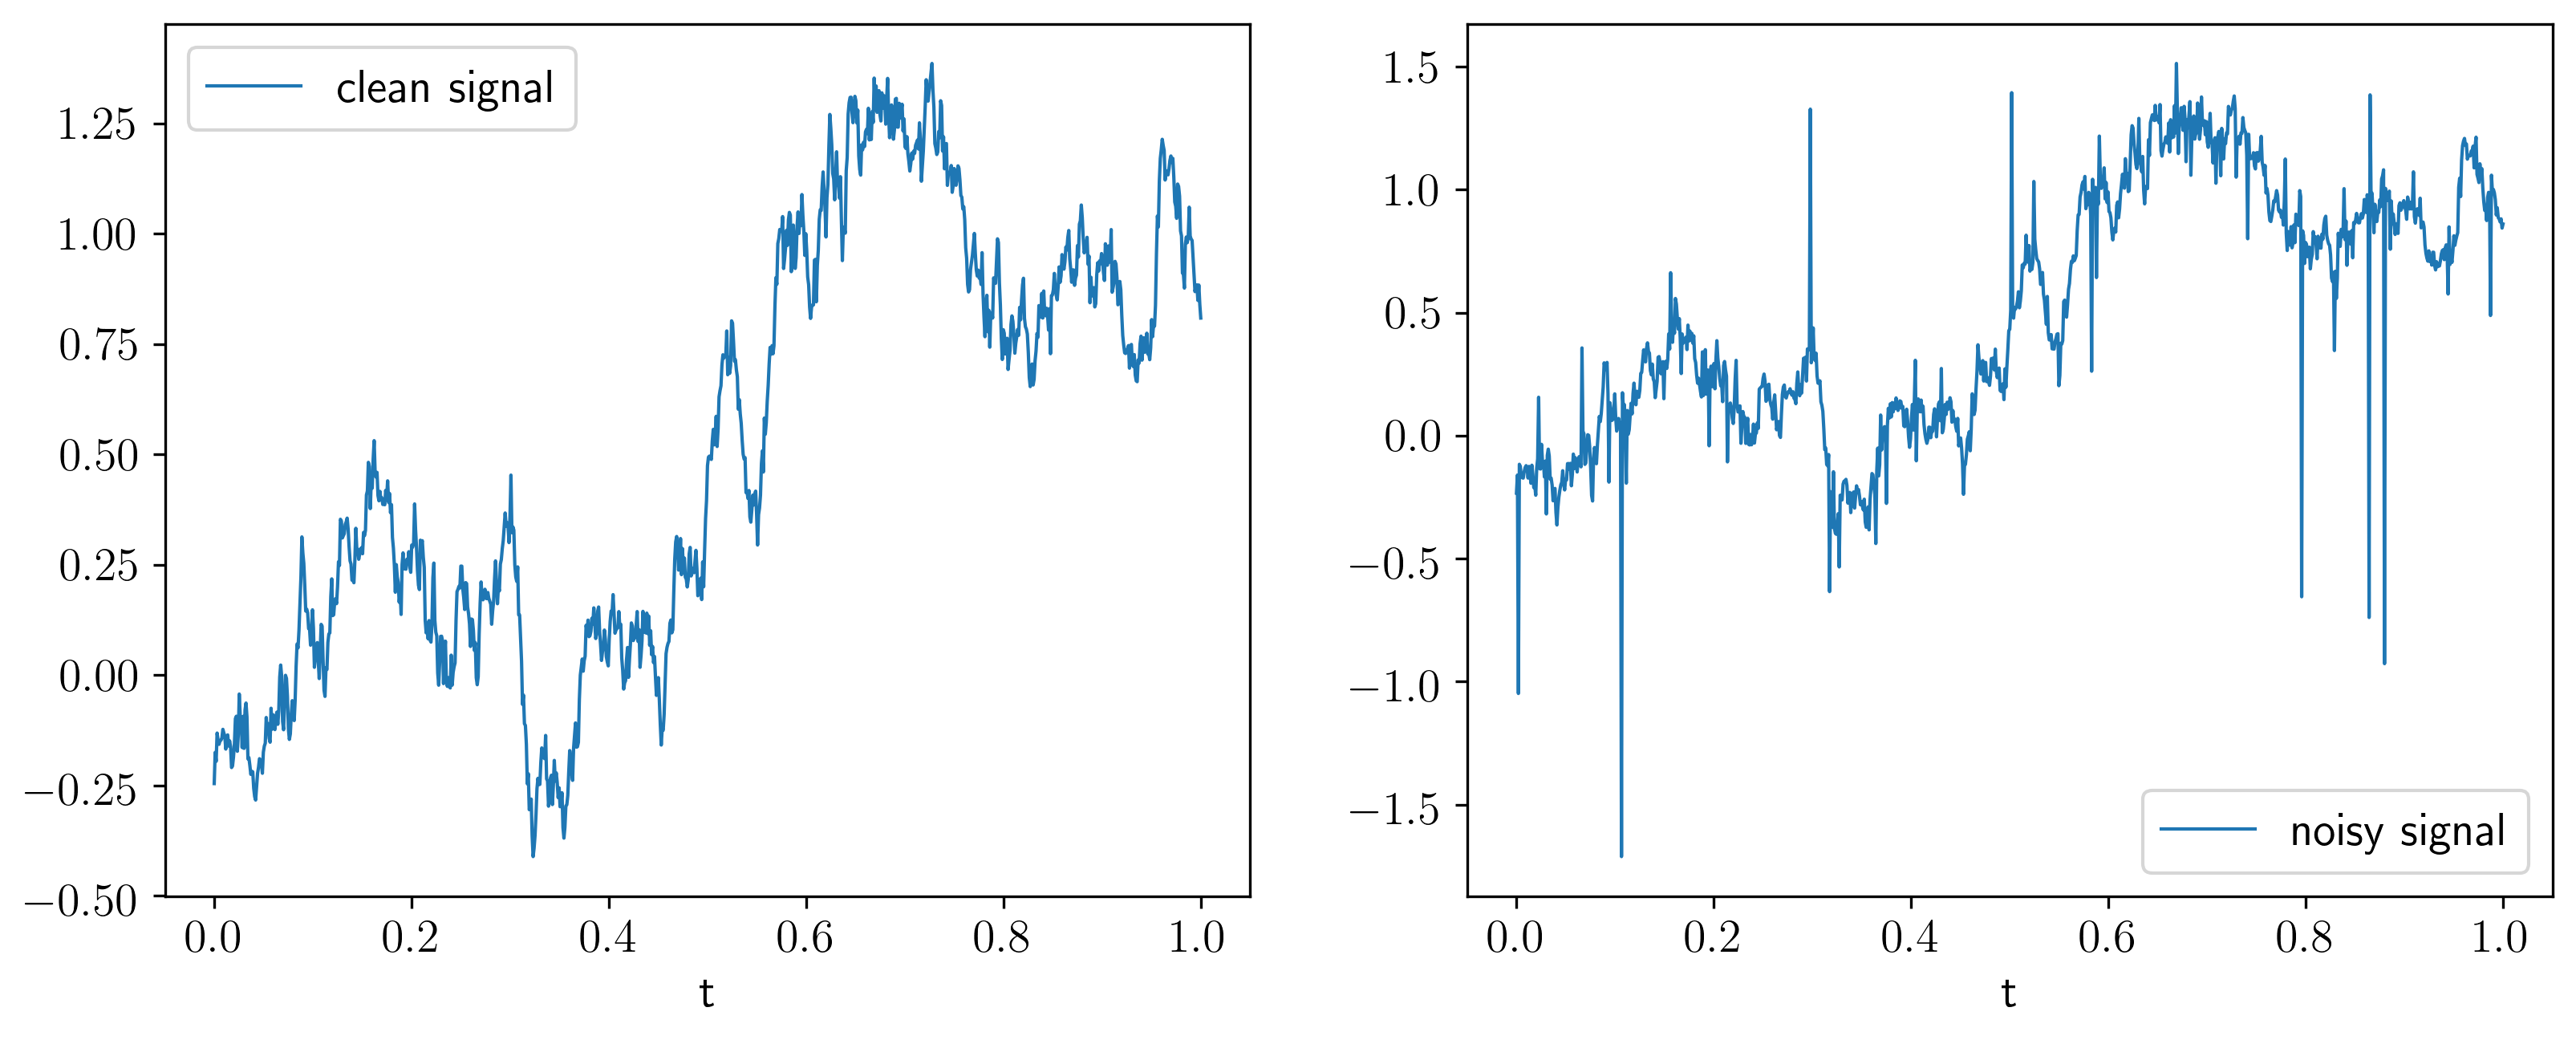
\includegraphics[width=\textwidth]{figures/10_cnoisy.png}
    \caption{Чистый и зашумленный сигналы. Шум распределен по Коши.}
    \label{fig:10_cnoisy}
\end{figure}
\begin{figure}[H]
    \centering
    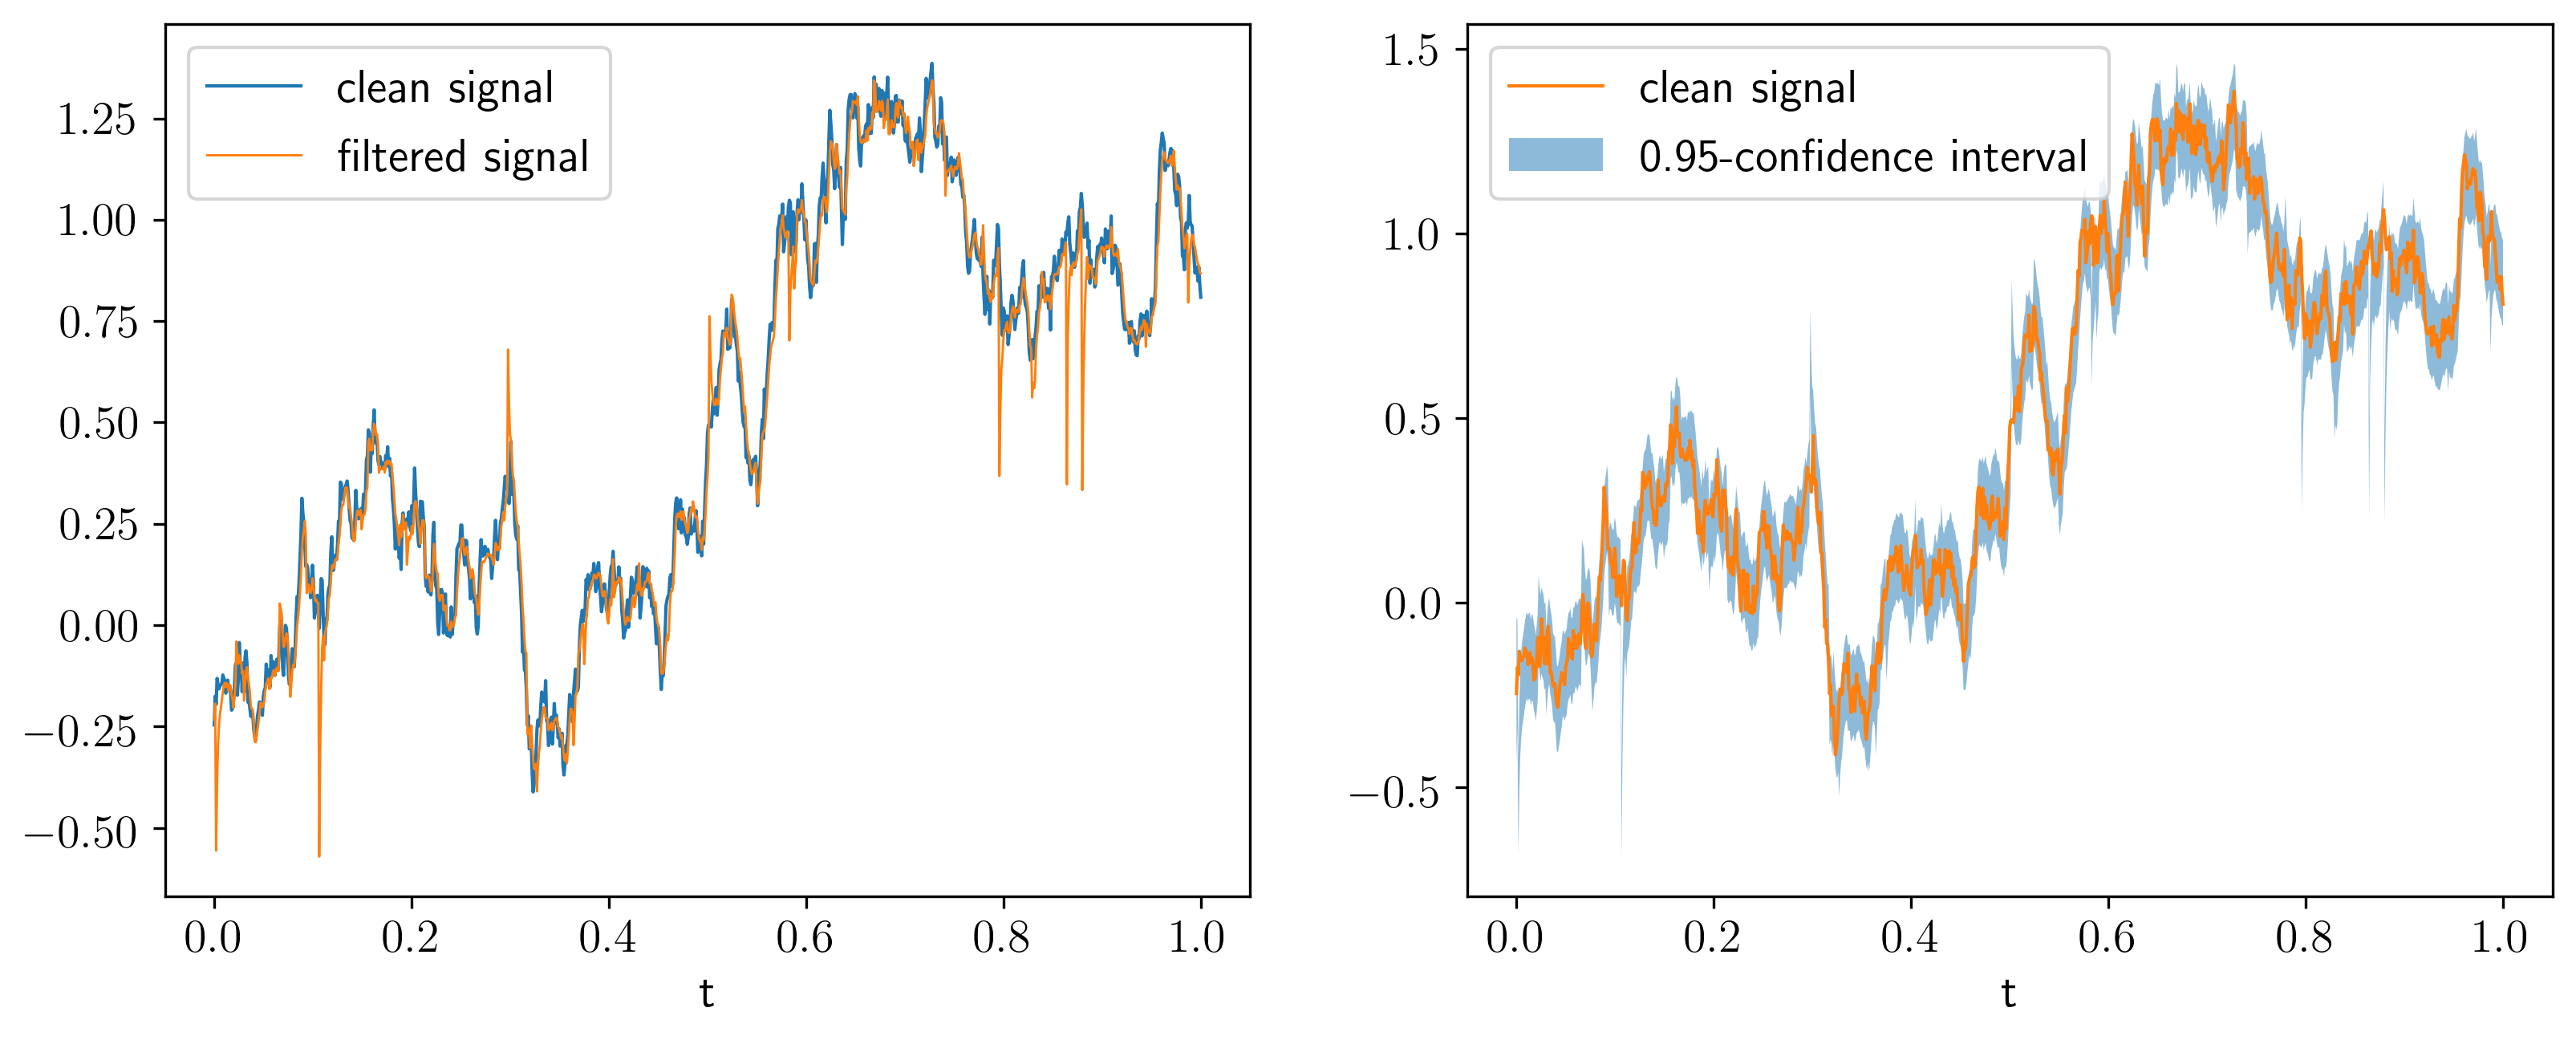
\includegraphics[width=\textwidth]{figures/10_cfiltered.png}
    \caption{Результат фильтрации.}
    \label{fig:10_сfiltered}
\end{figure}

\section{Задание 11}
\subsection{Постановка задачи}
Построить двумерное пуассоновское поле, отвечающее сложному пуассоновскому процессу:
\begin{enumerate}
	\item Первая интерпретация: система массового обслуживания. При этом, первая координата поля --- время поступления заявки в СМО (равномерное распределение), вторая --- время ее обслуживания (распределение $\chi^2$ с 10 степенями свободы).
	\item Вторая интерпретация: система массового обслуживания с циклической активностью $\lambda(1 + \cos(t))$ и единичными скачками. Свести данную задачу при помощи метода Льюиса и Шедлеара к моделированию двумерного пуассоновского поля, где первая координата имеет равномерное распределение, а вторая --- распределение Бернулли.
	\item Третья интерпретация: работа страховой компании. Первая координата --- момент наступления страхового случая (равномерное распределение), вторая координата --- величина ущерба (распределение Парето). Поступление капитала по времени линейно со скоростью $c > 0$, начальный капитал $W > 0$.
	\item Для каждой системы рассмотреть все возможные случаи поведения системы в зависимости от значения параметров.
\end{enumerate}

\subsection{Теоретическая часть}

Рассмотрим первую интерпретацию.
Так как время поступления заявки имеет равномерное распределение,
то мы имеем дело с пуассоовким процессом.
Обозначим за $\lambda$ интенсивность данного процесса. 
Тогда за единицу времени в СМО поступает в среднем  $\lambda$ заявок.
Так как время обработки заявки имеер распределение $\chi^2(10)$, 
среднее время обработки заявки в СМО составляет $1 / 10$.
Таким образом, возможно 3 варианта эволюции СМО:
\begin{enumerate}
    \item $\lambda < 1 / 10$~--- заявки в среднем обрабатываются быстрее, чем поступают новые, СМО простаивает.
    \item $\lambda = 1 / 10$~--- средняя интенсивность поступления заявом совпадает с интенсивностью их обработки. 
        Процесс находится в равновесии.
    \item $\lambda > 1 / 10$~--- СМО не успевает обрабатывать заявки, возникает растущая очередь.
\end{enumerate} 

Метод Льюиса и Шедлеара для моделирования Пуассоновского процесса с интенсивностью $\lambda(t)$ очень похож на метод элиминации фон Неймана.
Пусть $\lambda(t)  \le \lambda^*\ \forall t \ge 0$.
Затем в каждый момент поступления заявки $t_i$ с вероятностью  $1 - \lambda(t_i) \big/ \lambda^*$ отбрасываем заявку.
В результате получается процесс с нужной интенсивностью.
В задании  $\lambda^* = 2\lambda$. 
Так как среднее значение интенсивности равно $\lambda$, случаи те же, что и в 1-й интерпретации.

Работу страховой компании будем моделировать с помощью следующего процесса:
$$
X(t) = W + ct - \sum\limits_{n=0}^{N(t)} \xi_n,
$$
где $N(t)$ — пуассоновский процесс с интенсивностью $\lambda$, $W$~--- начальный капитал,
$c$~--- скорость поступления капитала, а $\xi_n$ имеет распределение Парето с показателем $b$.
Распределение Парето имеет функцию распределения 
\[
F_{\xi_n}(x) = 
    \begin{cases}
        0, & x < 1, \\
        1 - x^{-b}, & x \ge 1.
    \end{cases} 
\] 
При $b > 1$ матемаическое ожидание существует и $\mathbb{E}\xi_n = b \big/ (b - 1)$ и $\mathbb{E} X(t) = W + ct +\lambda t b \big/ (b - 1)$.
Соответственно, критическое значение $b^* = c \big/ (c - \lambda)$.
Если хвост тяжелее, то капитал в среднем будет расти, если легче, то убывать.

\subsection{Результаты работы программы}
\begin{figure}[H]
    \centering
    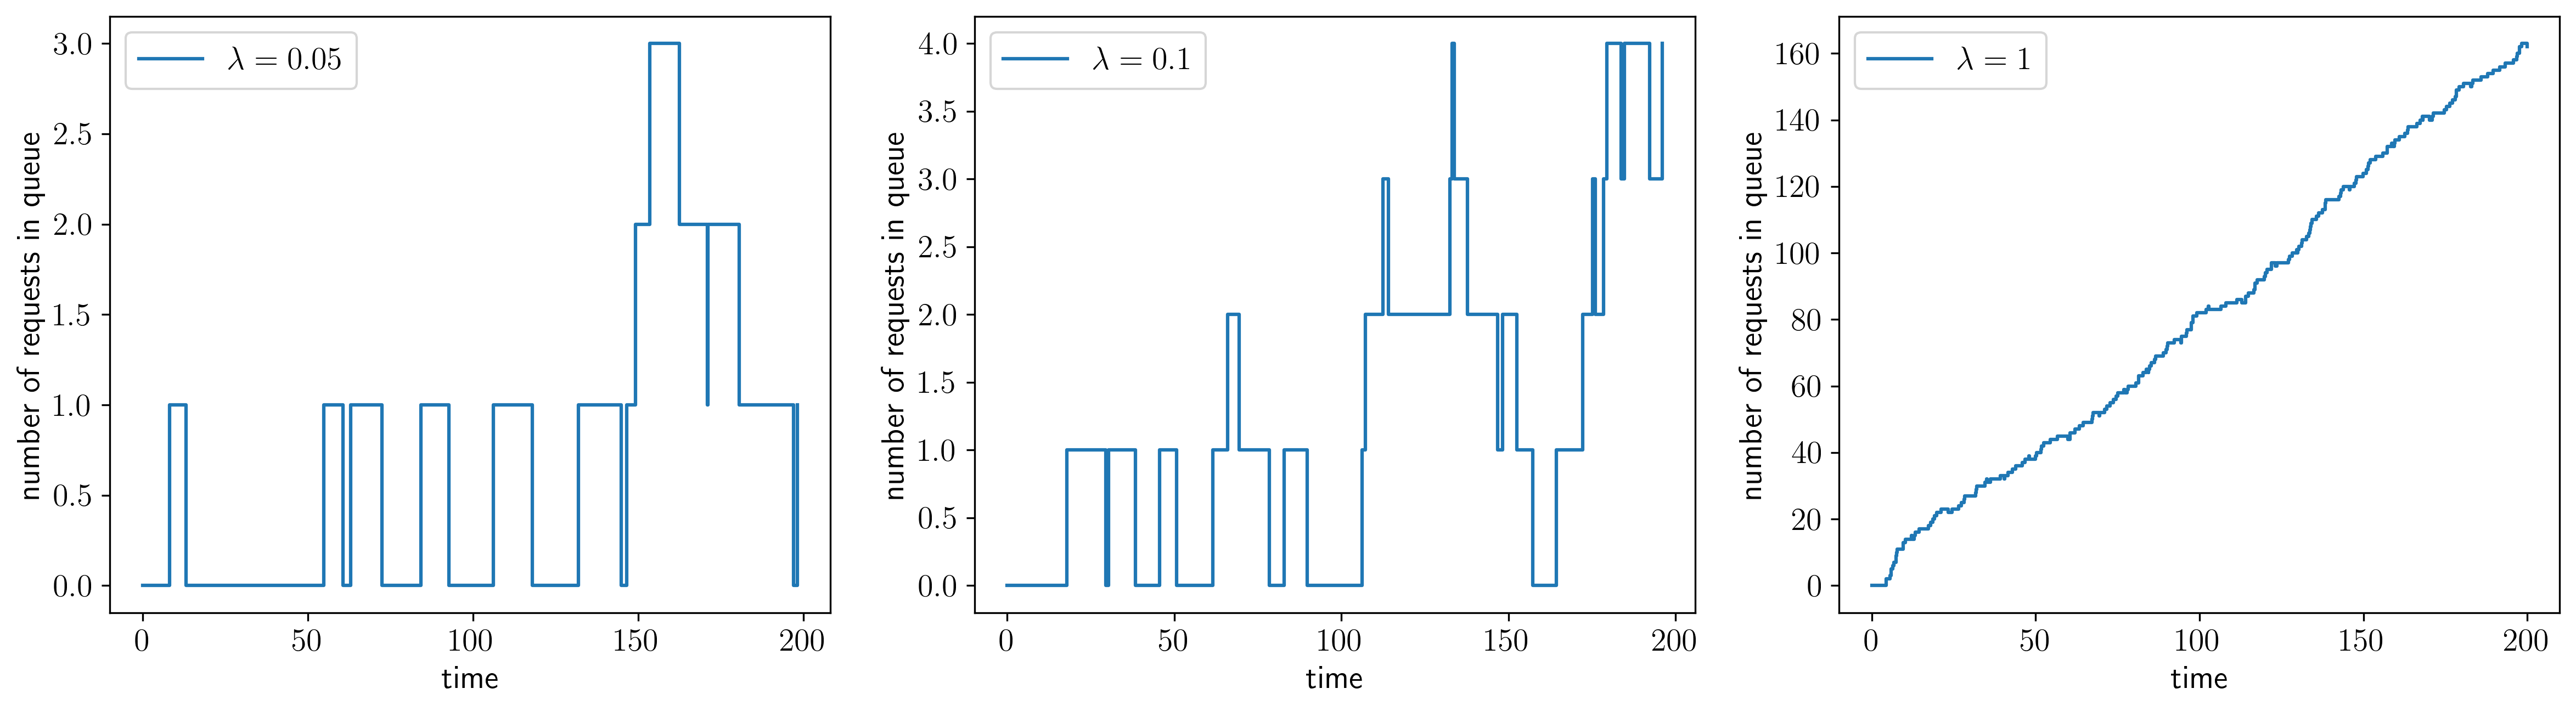
\includegraphics[width=\textwidth]{figures/11_vanilla.png}
    \caption{Моделирование СМО с постоянной активностью при разных интенсивностях поступления заявок.}
    \label{fig:11_vanilla}
\end{figure}
\begin{figure}[H]
    \centering
    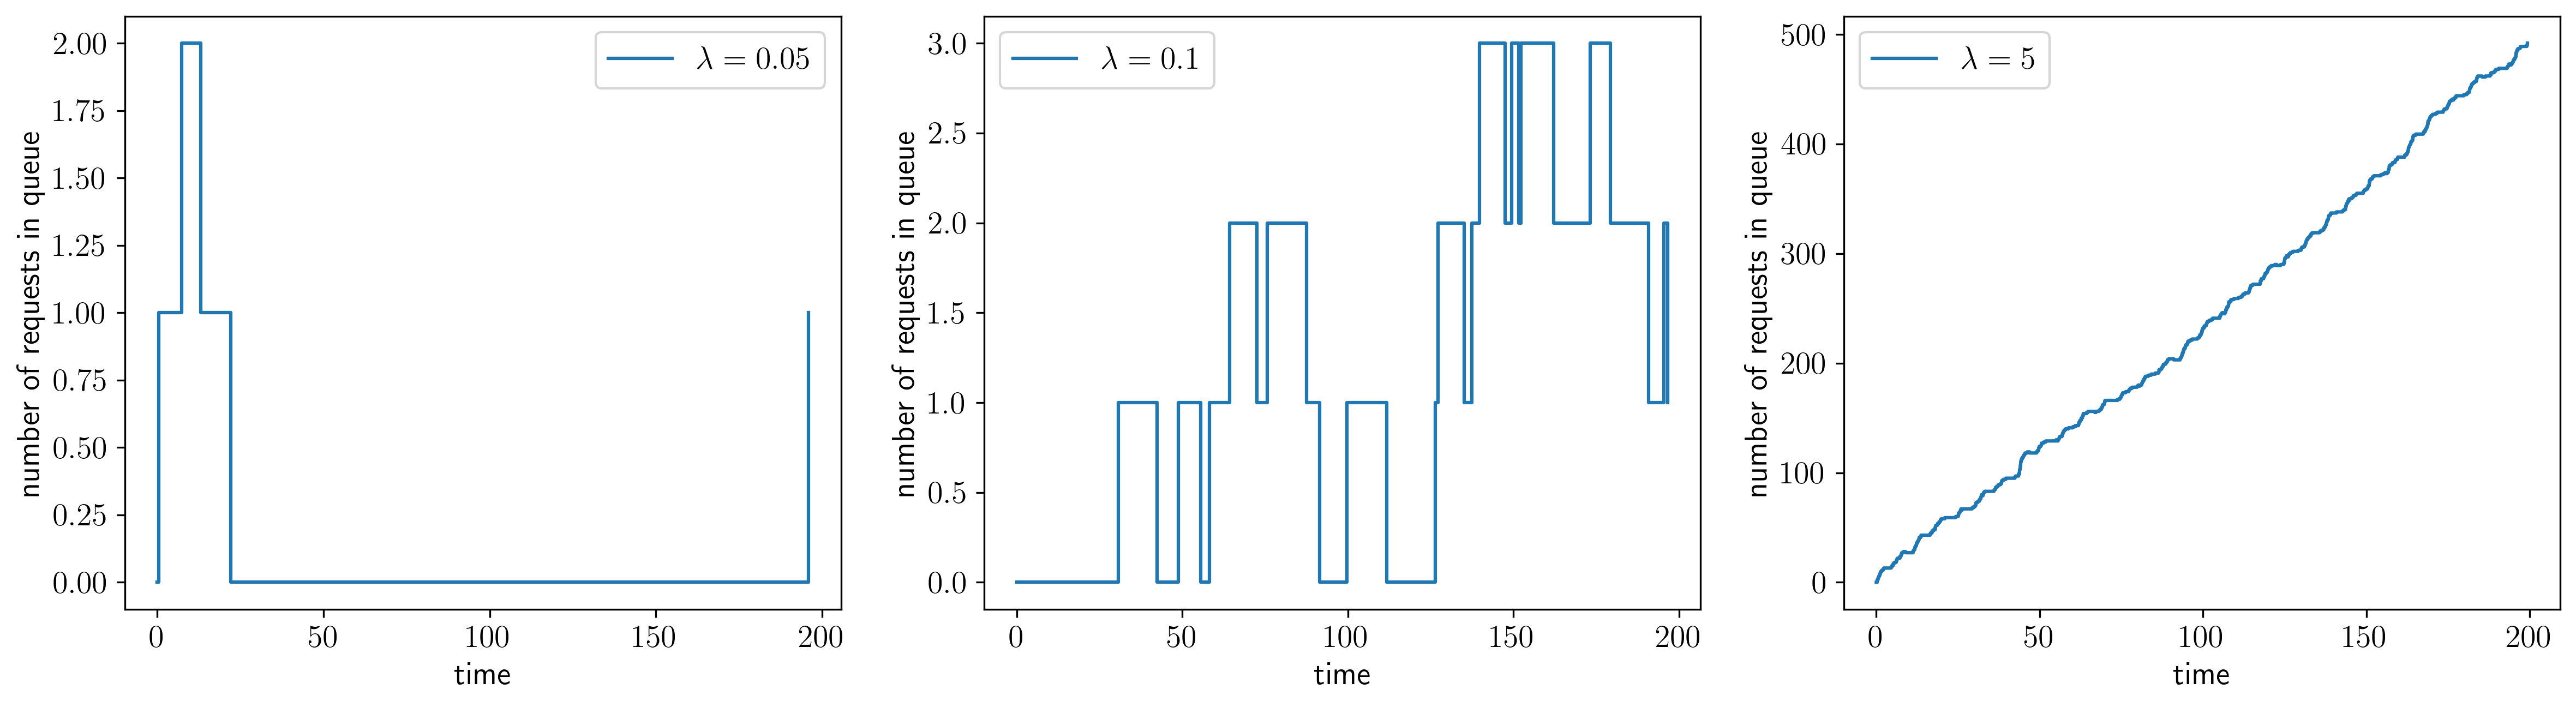
\includegraphics[width=\textwidth]{figures/11_cyclic.png}
    \caption{Моделирование СМО с циклической активностью при разных интенсивностях поступления заявок.}
    \label{fig:11_cyclic}
\end{figure}
\begin{figure}[H]
    \centering
    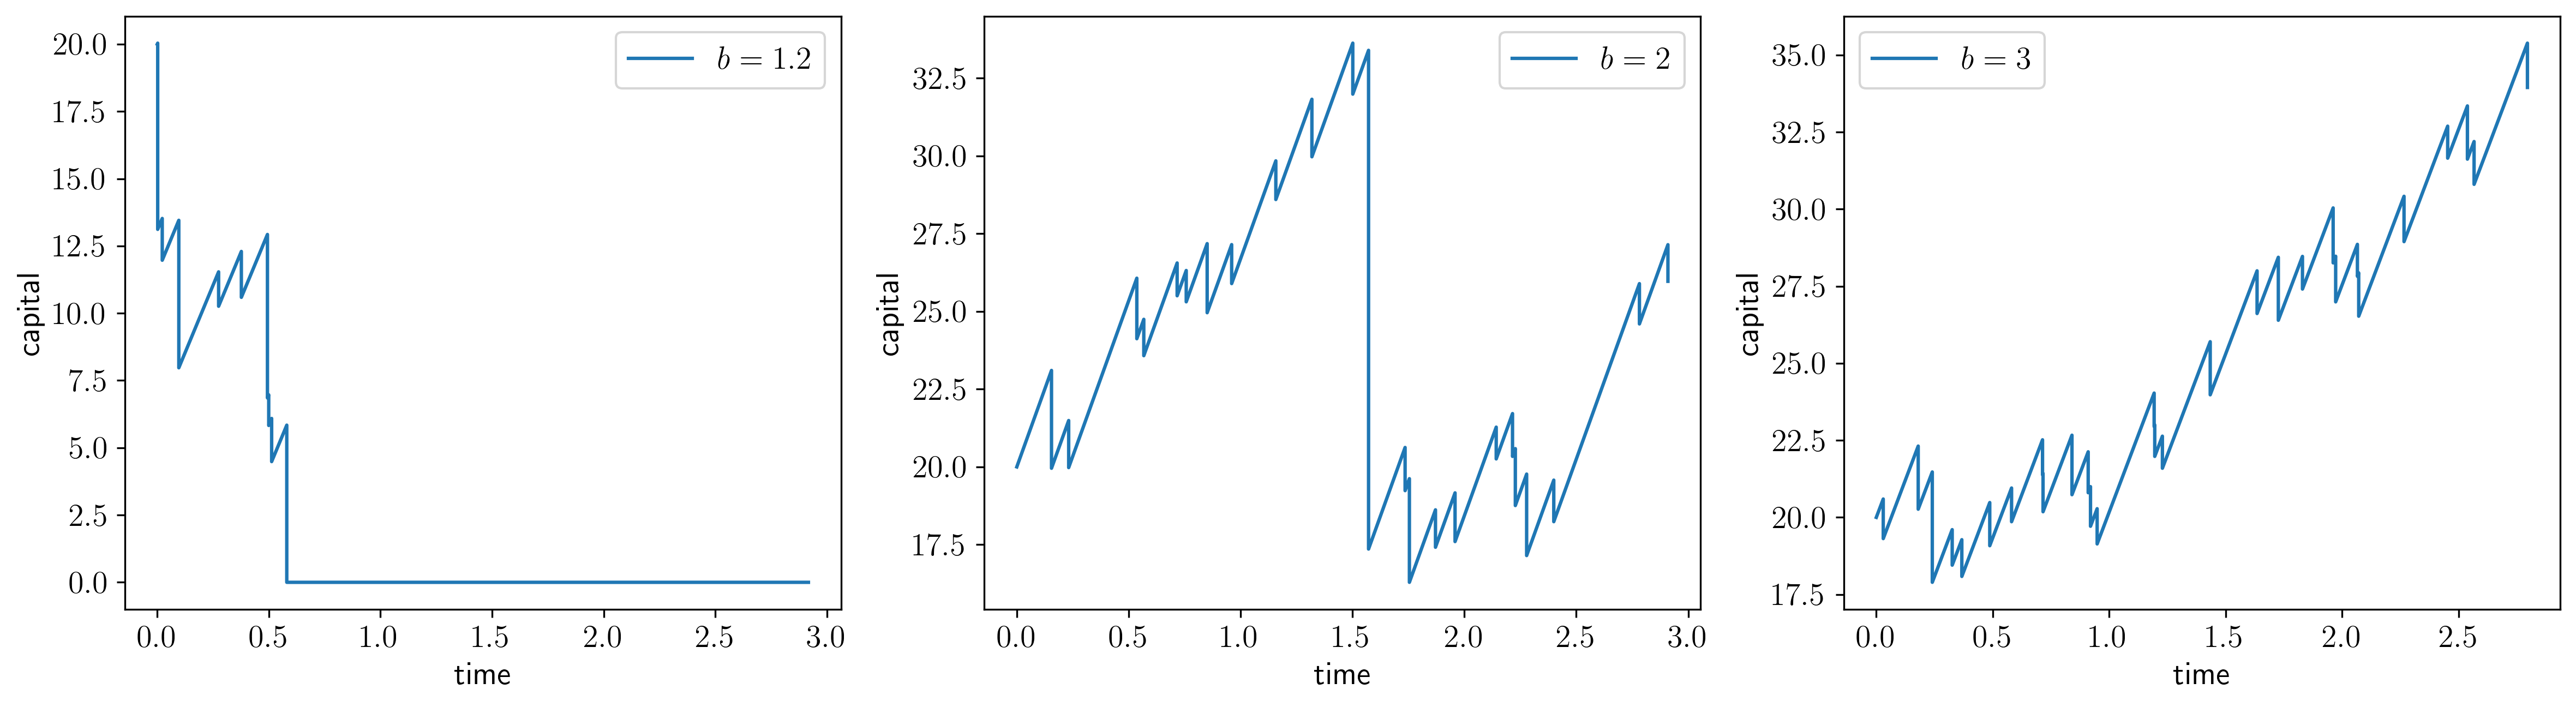
\includegraphics[width=\textwidth]{figures/11_insur.png}
    \caption{Моделирование работы страховой компании. Параметры $W = 20$ и $c = 20$. Интенсивность страховых случаев $\lambda = 10$.}
    \label{fig:11_insur}
\end{figure}

\newpage

\bibliographystyle{utf8gost705u}
\bibliography{biblio}
 \end{document} 
